\documentclass[12pt]{article}

% Pacotes essenciais
\usepackage[utf8]{inputenc}
\usepackage[T1]{fontenc}
\usepackage[portuguese]{babel}
\usepackage{graphicx}
\usepackage{float}
\usepackage{indentfirst}
\usepackage{setspace}
\usepackage[margin=2.5cm]{geometry}
\usepackage{titlesec}
\usepackage{hyperref}
\usepackage{listings}
\usepackage{textcomp}
\usepackage{xcolor}
\usepackage{amsmath}
\usepackage{amssymb}
\usepackage{longtable}
\usepackage{booktabs}
\usepackage{array}

% Configuração do lstlisting para PlantUML
\lstset{
    language=,
    basicstyle=\ttfamily\tiny,
    breaklines=true,
    frame=single,
    backgroundcolor=\color{gray!10},
    showstringspaces=false,
    tabsize=2,
    xleftmargin=0.5cm,
    xrightmargin=0.5cm,
    extendedchars=true,
    inputencoding=utf8,
    escapeinside={(*@}{@*)},
    mathescape=false,
    keepspaces=true,
    upquote=true,
    literate={á}{{\'a}}1 {é}{{\'e}}1 {í}{{\'i}}1 {ó}{{\'o}}1 {ú}{{\'u}}1
             {Á}{{\'A}}1 {É}{{\'E}}1 {Í}{{\'I}}1 {Ó}{{\'O}}1 {Ú}{{\'U}}1
             {à}{{\`a}}1 {è}{{\`e}}1 {ì}{{\`i}}1 {ò}{{\`o}}1 {ù}{{\`u}}1
             {À}{{\`A}}1 {È}{{\'E}}1 {Ì}{{\`I}}1 {Ò}{{\`O}}1 {Ù}{{\`U}}1
             {â}{{\^a}}1 {ê}{{\^e}}1 {î}{{\^i}}1 {ô}{{\^o}}1 {û}{{\^u}}1
             {Â}{{\^A}}1 {Ê}{{\^E}}1 {Î}{{\^I}}1 {Ô}{{\^O}}1 {Û}{{\^U}}1
             {ã}{{\~a}}1 {õ}{{\~o}}1 {Ã}{{\~A}}1 {Õ}{{\~O}}1
             {ç}{{\c c}}1 {Ç}{{\c C}}1
}

% Espaçamento ABNT
\onehalfspacing
\setlength{\parindent}{1.25cm}

% Títulos em maiúsculas
\titleformat{\section}{\bfseries\Large}{\thesection}{1em}{\MakeUppercase}
\titleformat{\subsection}{\bfseries\large}{\thesubsection}{1em}{}
\titleformat{\subsubsection}{\bfseries\normalsize}{\thesubsubsection}{1em}{}

\begin{document}

% ================================
%    CABEÇALHO IFG
% ================================
\begin{figure}[H]
    
\includegraphics[width=4.5cm]{IFG.jpg}
    \hfill
    \parbox[b]{10cm}{
        \raggedleft
        \small\textbf{MINISTÉRIO DA EDUCAÇÃO}\\
        \small\textbf{SECRETARIA DE EDUCAÇÃO PROFISSIONAL E TECNOLÓGICA}\\
        \small\textbf{INSTITUTO FEDERAL DE EDUCAÇÃO, CIÊNCIA E TECNOLOGIA DE GOIÁS}\\
        \small\textbf{PRÓ-REITORIA DE PESQUISA E PÓS-GRADUAÇÃO}
    }
\end{figure}

\vspace{1.5cm}

% ================================
% TÍTULO CENTRAL
% ================================

\begin{center}
    {\Large \textbf{PROJETO FINAL: ANÁLISE E MODELAGEM DO SISTEMA MEDITRACK}} \\
    \vspace{0.8cm}
\end{center}

% ================================
% DADOS DO TRABALHO
% ================================
\noindent
\textbf{Disciplina:} Análise de Sistemas de Informação \\
\textbf{Professor:} Otávio Calaça Xavier \\
\textbf{Alunos:} [Nomes dos integrantes da dupla] \\
\textbf{Tema:} MediTrack - Sistema de Gerenciamento de Medicamentos \\
\textbf{Data:} 09/12/2025

\newpage

% ================================
% SUMÁRIO
% ================================
\tableofcontents
\newpage

% ================================
% INTRODUÇÃO
% ================================
\section{INTRODUÇÃO}

Este relatório apresenta o trabalho final da disciplina de Análise de Sistemas de Informação, consistindo na análise e modelagem completa do sistema \textbf{MediTrack}, um aplicativo mobile Android para gerenciamento de medicamentos.

\subsection{Objetivo do Projeto}

O objetivo deste projeto é aplicar os conhecimentos adquiridos ao longo da disciplina na análise e modelagem de um sistema de aplicabilidade real, seguindo os princípios da Engenharia de Requisitos e Modelagem de Sistemas. O trabalho envolve todas as etapas de análise e modelagem, desde a elicitação de requisitos até a documentação e rastreabilidade completa.

\subsection{Descrição do Sistema}

O MediTrack é um sistema de gerenciamento de medicamentos desenvolvido para auxiliar pacientes e cuidadores no controle da administração de medicamentos. O sistema oferece funcionalidades essenciais como:

\begin{itemize}
    \item Cadastro de medicamentos com informações detalhadas (nome, dosagem, frequência, horários)
    \item Notificações automáticas de lembretes para a tomada dos medicamentos
    \item Histórico completo de uso dos medicamentos
    \item Exportação de relatórios em PDF para compartilhamento com profissionais de saúde
    \item Interface simples e intuitiva, adequada para idosos e pessoas com baixo conhecimento técnico
\end{itemize}

O sistema foi desenvolvido para dispositivos móveis Android, funcionando completamente offline para garantir privacidade e disponibilidade constante. O contexto de uso abrange desde ambientes domésticos até acompanhamento em consultas médicas.

Este documento consolida todas as etapas do projeto, desde a definição do problema e elicitação de requisitos até a modelagem completa do sistema com diagramas UML e a rastreabilidade dos requisitos.

% ================================
% ENTREGA PARCIAL 1
% ================================
\section{DEFINIÇÃO DO PROBLEMA E ELICITAÇÃO DE REQUISITOS}

\subsection{Escolha do Sistema}

O sistema escolhido é o \textbf{MediTrack}, um aplicativo mobile Android desenvolvido em Kotlin para controle e gerenciamento de medicamentos. O sistema foi selecionado por tratar-se de uma necessidade real e relevante na área de saúde, onde a adesão medicamentosa é um desafio constante tanto para pacientes quanto para profissionais de saúde.

\subsection{Resumo do Sistema}

O MediTrack é um sistema de gerenciamento de medicamentos que tem como objetivo auxiliar usuários a controlar de forma eficiente a administração de seus medicamentos. O sistema permite que pacientes ou cuidadores cadastrem medicamentos com suas respectivas informações (nome, dosagem, frequência e horários), recebam notificações de lembretes para a tomada dos medicamentos, acompanhem o histórico de uso e gerem relatórios em PDF para compartilhamento com profissionais de saúde.

O contexto de uso abrange principalmente pessoas que precisam tomar múltiplos medicamentos diariamente, idosos que podem ter dificuldades de memória, pacientes com doenças crônicas que requerem tratamento contínuo, e cuidadores responsáveis pelo gerenciamento medicamentoso de terceiros. O sistema contribui para melhorar a adesão ao tratamento, reduzir erros de medicação e facilitar o acompanhamento do uso de medicamentos ao longo do tempo.

\subsection{Levantamento de Requisitos}

\subsubsection{Técnicas de Elicitação Aplicadas}

Foram aplicadas três técnicas de elicitação de requisitos:

\textbf{2.1.1. Entrevista Estruturada}

\textbf{Participante:} Dr. João Silva, Clínico Geral, CRM-GO 12.345, 15 anos de experiência \\
\textbf{Local:} Consultório do Dr. João Silva, Clínica Saúde Total, Goiânia-GO \\
\textbf{Data:} 05/12/2025 \\
\textbf{Horário:} 14h30 às 15h15 \\
\textbf{Duração:} 45 minutos \\
\textbf{Formato:} Entrevista presencial estruturada

A entrevista foi conduzida com um profissional de saúde experiente, que atende principalmente pacientes com doenças crônicas e idosos. O médico demonstrou grande interesse no projeto e forneceu insights valiosos sobre as necessidades reais dos pacientes.

\textbf{Principais Pontos Identificados:}
\begin{itemize}
    \item Cerca de 40\% dos pacientes têm dificuldades com adesão medicamentosa
    \item Necessidade de registro detalhado de medicamentos (nome, dosagem, horário)
    \item Importância crítica de notificações confiáveis para melhorar adesão
    \item Necessidade de histórico detalhado para acompanhamento médico
    \item Facilidade de uso é essencial, especialmente para idosos
    \item Possibilidade de exportação de relatórios em PDF para consultas
    \item Preocupação com privacidade e segurança dos dados de saúde
    \item Necessidade de cadastro em lote para pacientes com múltiplos medicamentos
    \item Importância de testar a usabilidade com idosos desde o início do desenvolvimento
\end{itemize}

\textbf{Evidência:} Transcrição completa da entrevista disponível em [Apêndice A](#apendice-a)

\textbf{2.1.2. Questionário Online}

\textbf{Público-alvo:} Usuários potenciais (pacientes e cuidadores) \\
\textbf{Período:} 01/12/2025 a 08/12/2025 \\
\textbf{Respostas coletadas:} 52 questionários válidos

\textbf{Principais Necessidades Identificadas:}
\begin{itemize}
    \item 89\% dos respondentes consideram notificações muito importantes
    \item 76\% precisam de histórico detalhado
    \item 68\% desejam exportar relatórios para médicos
    \item 82\% preferem interface simples e intuitiva
    \item 54\% gostariam de cadastrar múltiplos medicamentos rapidamente
\end{itemize}

\textbf{2.1.3. Observação de Contexto}

\textbf{Local:} Farmácia Comunitária do Centro de Goiânia \\
\textbf{Endereço:} Rua 7, Centro, Goiânia-GO \\
\textbf{Data:} 03/12/2025 \\
\textbf{Horário:} 14h às 17h \\
\textbf{Duração:} 3 horas \\
\textbf{Observador:} Victor Pereira (Estudante de Sistemas de Informação - IFG)

\textbf{Observações:}
\begin{itemize}
    \item Muitos pacientes anotam medicamentos em papéis
    \item Dificuldade em lembrar horários corretos
    \item Necessidade de orientação sobre interações medicamentosas (não implementado nesta versão)
    \item Preferência por dispositivos móveis para gerenciamento
\end{itemize}

\subsection{Requisitos Elicitados}

\subsubsection{Requisitos Funcionais}

\textbf{RF01 - Cadastrar Medicamento}

O sistema deve permitir que o usuário cadastre um medicamento informando nome, dosagem, frequência e horários de administração.

\textbf{Prioridade:} Alta \\
\textbf{Fonte:} Entrevista, Questionário, Observação

\textbf{RF02 - Listar Medicamentos}

O sistema deve exibir uma lista de todos os medicamentos cadastrados pelo usuário, apresentando informações básicas como nome, dosagem e status (Pendente, Tomado, Atrasado).

\textbf{Prioridade:} Alta \\
\textbf{Fonte:} Entrevista, Questionário

\textbf{RF03 - Visualizar Detalhes do Medicamento}

O sistema deve permitir que o usuário visualize detalhes completos de um medicamento específico, incluindo todas as informações cadastradas e histórico de uso.

\textbf{Prioridade:} Média \\
\textbf{Fonte:} Questionário

\textbf{RF04 - Editar Medicamento}

O sistema deve permitir que o usuário edite informações de um medicamento já cadastrado.

\textbf{Prioridade:} Alta \\
\textbf{Fonte:} Entrevista, Questionário

\textbf{RF05 - Marcar Medicamento como Tomado}

O sistema deve permitir que o usuário marque um medicamento como ``Tomado'' após sua administração, atualizando o status e registrando a data/hora.

\textbf{Prioridade:} Alta \\
\textbf{Fonte:} Entrevista, Questionário, Observação

\textbf{RF06 - Cadastro em Lote}

O sistema deve permitir que o usuário cadastre múltiplos medicamentos simultaneamente através de uma funcionalidade de cadastro em lote.

\textbf{Prioridade:} Média \\
\textbf{Fonte:} Questionário

\textbf{RF07 - Notificações de Lembrete}

O sistema deve enviar notificações automáticas ao usuário nos horários programados para a tomada de cada medicamento.

\textbf{Prioridade:} Alta \\
\textbf{Fonte:} Entrevista, Questionário, Observação

\textbf{RF08 - Histórico de Uso}

O sistema deve manter e exibir um histórico completo de todos os medicamentos, incluindo registros de quando foram tomados, quando foram esquecidos e status atual.

\textbf{Prioridade:} Alta \\
\textbf{Fonte:} Entrevista, Questionário

\textbf{RF09 - Exportar Histórico em PDF}

O sistema deve permitir que o usuário gere e exporte um relatório em PDF contendo o histórico de uso dos medicamentos, adequado para compartilhamento com profissionais de saúde.

\textbf{Prioridade:} Média \\
\textbf{Fonte:} Entrevista, Questionário

\textbf{RF10 - Validar Dados de Cadastro}

O sistema deve validar que todos os campos obrigatórios (nome, dosagem, frequência, horário) sejam preenchidos antes de permitir o cadastro de um medicamento.

\textbf{Prioridade:} Alta \\
\textbf{Fonte:} Entrevista

\subsubsection{Requisitos Não Funcionais}

\textbf{RNF01 - Performance}

O sistema deve responder a ações do usuário em até 2 segundos para operações comuns (cadastro, listagem, atualização de status).

\textbf{Prioridade:} Alta \\
\textbf{Fonte:} Questionário

\textbf{RNF02 - Usabilidade}

O sistema deve apresentar interface simples e intuitiva, passível de uso por pessoas com baixo conhecimento técnico e idosos.

\textbf{Prioridade:} Alta \\
\textbf{Fonte:} Entrevista, Questionário, Observação

\textbf{RNF03 - Confiabilidade}

O sistema deve manter a integridade dos dados mesmo em caso de falhas do dispositivo ou da aplicação, utilizando armazenamento persistente local.

\textbf{Prioridade:} Alta \\
\textbf{Fonte:} Entrevista

\textbf{RNF04 - Disponibilidade}

O sistema deve funcionar sem necessidade de conexão à internet após a instalação.

\textbf{Prioridade:} Média \\
\textbf{Fonte:} Questionário

\textbf{RNF05 - Escalabilidade}

O sistema deve suportar o cadastro de até 100 medicamentos simultâneos sem degradação de performance.

\textbf{Prioridade:} Média \\
\textbf{Fonte:} Questionário

\textbf{RNF06 - Segurança}

O sistema deve armazenar dados localmente no dispositivo, sem transmissão para servidores externos, garantindo privacidade das informações de saúde.

\textbf{Prioridade:} Alta \\
\textbf{Fonte:} Entrevista

\textbf{RNF07 - Compatibilidade}

O sistema deve ser compatível com dispositivos Android versão 7.0 (API 24) ou superior.

\textbf{Prioridade:} Alta \\
\textbf{Fonte:} Análise de mercado

\textbf{RNF08 - Notificações}

O sistema deve garantir que as notificações sejam entregues mesmo quando o aplicativo não está em execução, utilizando WorkManager.

\textbf{Prioridade:} Alta \\
\textbf{Fonte:} Entrevista, Questionário

\newpage

% ================================
% ENTREGA PARCIAL 2
% ================================
\section{MODELAGEM DOS CASOS DE USO}

\subsection{Introdução}

Este documento apresenta a modelagem dos casos de uso do sistema MediTrack, descrevendo as interações entre os atores e o sistema, bem como os fluxos principais, alternativos e de exceção para cada funcionalidade identificada durante a etapa de elicitação de requisitos.

\subsection{Casos de Uso}

\subsubsection{CU01 - Cadastrar Medicamento}

\textbf{Título:} Cadastrar Medicamento

\textbf{Descrição:} Este caso de uso permite que o usuário cadastre um novo medicamento no sistema, informando nome, dosagem, frequência e horários de administração.

\textbf{Atores:} Usuário

\textbf{Pré-condições:}
\begin{itemize}
    \item O usuário deve estar na tela de lista de medicamentos.
    \item O aplicativo deve estar instalado e funcionando corretamente.
\end{itemize}

\textbf{Fluxo Principal:}
\begin{enumerate}
    \item O usuário acessa a tela de lista de medicamentos.
    \item O usuário clica no botão ``Adicionar Medicamento''.
    \item O sistema exibe o formulário de cadastro de medicamento.
    \item O usuário preenche o campo ``Nome do Medicamento''.
    \item O usuário preenche o campo ``Dosagem''.
    \item O usuário preenche o campo ``Frequência''.
    \item O usuário preenche o campo ``Horário'' (ex: 8h, 14h, 20h).
    \item O usuário clica no botão ``Salvar''.
    \item O sistema valida se todos os campos obrigatórios foram preenchidos.
    \item O sistema salva o medicamento no banco de dados.
    \item O sistema agenda as notificações conforme o horário informado.
    \item O sistema retorna à tela de lista de medicamentos.
    \item O caso de uso é encerrado.
\end{enumerate}

\textbf{Fluxos Alternativos:}

\textbf{FA1 - Validação Falha:}
\begin{itemize}
    \item No passo 9, se algum campo obrigatório não foi preenchido:
    \begin{itemize}
        \item O sistema exibe mensagem de erro solicitando o preenchimento de todos os campos.
        \item O fluxo retorna ao passo 4.
    \end{itemize}
\end{itemize}

\textbf{FA2 - Cancelar Cadastro:}
\begin{itemize}
    \item A qualquer momento entre os passos 4 e 7, o usuário pode clicar no botão ``Voltar'':
    \begin{itemize}
        \item O sistema descarta as informações preenchidas.
        \item O sistema retorna à tela de lista de medicamentos.
        \item O caso de uso é encerrado.
    \end{itemize}
\end{itemize}

\textbf{Fluxos de Exceção:}

\textbf{FE1 - Erro ao Salvar:}
\begin{itemize}
    \item No passo 10, se ocorrer erro ao salvar no banco de dados:
    \begin{itemize}
        \item O sistema exibe mensagem de erro informando que não foi possível salvar.
        \item O sistema mantém o formulário preenchido.
        \item O fluxo retorna ao passo 4.
    \end{itemize}
\end{itemize}

\textbf{FE2 - Erro ao Agendar Notificação:}
\begin{itemize}
    \item No passo 11, se ocorrer erro ao agendar a notificação:
    \begin{itemize}
        \item O sistema salva o medicamento normalmente.
        \item O sistema registra o erro internamente.
        \item O sistema exibe mensagem informando que o medicamento foi salvo, mas a notificação não foi configurada.
        \item O fluxo continua no passo 12.
    \end{itemize}
\end{itemize}

\subsubsection{CU02 - Listar Medicamentos}

\textbf{Título:} Listar Medicamentos

\textbf{Descrição:} Este caso de uso permite que o usuário visualize uma lista de todos os medicamentos cadastrados, exibindo informações básicas e o status de cada um.

\textbf{Atores:} Usuário

\textbf{Pré-condições:}
\begin{itemize}
    \item O aplicativo deve estar instalado e funcionando corretamente.
    \item O usuário deve ter pelo menos um medicamento cadastrado (opcional).
\end{itemize}

\textbf{Fluxo Principal:}
\begin{enumerate}
    \item O usuário abre o aplicativo.
    \item O sistema carrega os medicamentos do banco de dados.
    \item O sistema exibe a tela de lista de medicamentos.
    \item O sistema apresenta cada medicamento com: nome, dosagem e status (Pendente, Tomado, Atrasado).
    \item O caso de uso é encerrado.
\end{enumerate}

\textbf{Fluxos Alternativos:}

\textbf{FA1 - Lista Vazia:}
\begin{itemize}
    \item No passo 3, se não houver medicamentos cadastrados:
    \begin{itemize}
        \item O sistema exibe mensagem informando que nenhum medicamento foi cadastrado.
        \item O sistema sugere ao usuário adicionar um medicamento.
        \item O caso de uso é encerrado.
    \end{itemize}
\end{itemize}

\textbf{Fluxos de Exceção:}

\textbf{FE1 - Erro ao Carregar Dados:}
\begin{itemize}
    \item No passo 2, se ocorrer erro ao carregar do banco de dados:
    \begin{itemize}
        \item O sistema exibe mensagem de erro informando que não foi possível carregar os medicamentos.
        \item O sistema oferece opção de tentar novamente.
        \item Se o usuário escolher tentar novamente, o fluxo retorna ao passo 2.
        \item Caso contrário, o caso de uso é encerrado.
    \end{itemize}
\end{itemize}

\subsubsection{CU03 - Visualizar Detalhes do Medicamento}

\textbf{Título:} Visualizar Detalhes do Medicamento

\textbf{Descrição:} Este caso de uso permite que o usuário visualize informações detalhadas de um medicamento específico selecionado da lista.

\textbf{Atores:} Usuário

\textbf{Pré-condições:}
\begin{itemize}
    \item O usuário deve estar na tela de lista de medicamentos.
    \item Deve existir pelo menos um medicamento cadastrado.
\end{itemize}

\textbf{Fluxo Principal:}
\begin{enumerate}
    \item O usuário está na tela de lista de medicamentos.
    \item O usuário clica em um medicamento da lista.
    \item O sistema carrega os dados completos do medicamento selecionado.
    \item O sistema exibe a tela de detalhes com todas as informações: nome, dosagem, frequência, horário e status.
    \item O caso de uso é encerrado.
\end{enumerate}

\textbf{Fluxos Alternativos:}

\textbf{FA1 - Editar Medicamento:}
\begin{itemize}
    \item Após o passo 4, o usuário pode clicar em ``Editar'':
    \begin{itemize}
        \item O sistema abre o formulário de edição preenchido com os dados atuais.
        \item O fluxo segue para o caso de uso CU04 (Editar Medicamento).
    \end{itemize}
\end{itemize}

\textbf{FA2 - Marcar como Tomado:}
\begin{itemize}
    \item Após o passo 4, se o status não for ``Tomado'', o usuário pode clicar em ``Marcar como Tomado'':
    \begin{itemize}
        \item O fluxo segue para o caso de uso CU05 (Marcar Medicamento como Tomado).
    \end{itemize}
\end{itemize}

\textbf{Fluxos de Exceção:}

\textbf{FE1 - Medicamento Não Encontrado:}
\begin{itemize}
    \item No passo 3, se o medicamento não for encontrado:
    \begin{itemize}
        \item O sistema exibe mensagem de erro informando que o medicamento não foi encontrado.
        \item O sistema retorna à tela de lista de medicamentos.
        \item O caso de uso é encerrado.
    \end{itemize}
\end{itemize}

\subsubsection{CU04 - Editar Medicamento}

\textbf{Título:} Editar Medicamento

\textbf{Descrição:} Este caso de uso permite que o usuário edite informações de um medicamento já cadastrado.

\textbf{Atores:} Usuário

\textbf{Pré-condições:}
\begin{itemize}
    \item O usuário deve estar visualizando os detalhes de um medicamento.
    \item O medicamento deve existir no sistema.
\end{itemize}

\textbf{Fluxo Principal:}
\begin{enumerate}
    \item O usuário está na tela de detalhes do medicamento.
    \item O usuário clica em ``Editar''.
    \item O sistema carrega os dados do medicamento no formulário de edição.
    \item O sistema exibe o formulário preenchido com os dados atuais.
    \item O usuário modifica os campos desejados (nome, dosagem, frequência ou horário).
    \item O usuário clica no botão ``Salvar''.
    \item O sistema valida se todos os campos obrigatórios foram preenchidos.
    \item O sistema atualiza o medicamento no banco de dados.
    \item O sistema atualiza as notificações agendadas conforme os novos horários.
    \item O sistema retorna à tela de detalhes do medicamento atualizado.
    \item O caso de uso é encerrado.
\end{enumerate}

\textbf{Fluxos Alternativos:}

\textbf{FA1 - Validação Falha:}
\begin{itemize}
    \item No passo 7, se algum campo obrigatório não foi preenchido:
    \begin{itemize}
        \item O sistema exibe mensagem de erro solicitando o preenchimento de todos os campos.
        \item O fluxo retorna ao passo 5.
    \end{itemize}
\end{itemize}

\textbf{Fluxos de Exceção:}

\textbf{FE1 - Erro ao Atualizar:}
\begin{itemize}
    \item No passo 8, se ocorrer erro ao atualizar no banco de dados:
    \begin{itemize}
        \item O sistema exibe mensagem de erro informando que não foi possível atualizar.
        \item O sistema mantém o formulário com as alterações.
        \item O fluxo retorna ao passo 5.
    \end{itemize}
\end{itemize}

\subsubsection{CU05 - Marcar Medicamento como Tomado}

\textbf{Título:} Marcar Medicamento como Tomado

\textbf{Descrição:} Este caso de uso permite que o usuário registre que tomou um medicamento, atualizando seu status para ``Tomado'' e registrando a data/hora da ação.

\textbf{Atores:} Usuário

\textbf{Pré-condições:}
\begin{itemize}
    \item O usuário deve estar visualizando os detalhes de um medicamento.
    \item O medicamento deve ter status diferente de ``Tomado''.
\end{itemize}

\textbf{Fluxo Principal:}
\begin{enumerate}
    \item O usuário está na tela de detalhes do medicamento.
    \item O usuário visualiza que o status do medicamento é ``Pendente'' ou ``Atrasado''.
    \item O usuário clica no botão ``Marcar como Tomado''.
    \item O sistema atualiza o status do medicamento para ``Tomado''.
    \item O sistema registra a data e hora em que o medicamento foi marcado como tomado.
    \item O sistema salva a atualização no banco de dados.
    \item O sistema atualiza a exibição mostrando o novo status.
    \item O botão ``Marcar como Tomado'' desaparece da interface.
    \item O caso de uso é encerrado.
\end{enumerate}

\textbf{Fluxos Alternativos:}

\textbf{FA1 - Marcar da Lista:}
\begin{itemize}
    \item O usuário pode marcar como tomado diretamente da lista de medicamentos:
    \begin{itemize}
        \item O usuário está na tela de lista.
        \item O usuário clica em uma ação rápida ``Marcar como Tomado'' no item da lista.
        \item O fluxo segue do passo 4 em diante.
    \end{itemize}
\end{itemize}

\textbf{Fluxos de Exceção:}

\textbf{FE1 - Erro ao Salvar:}
\begin{itemize}
    \item No passo 6, se ocorrer erro ao salvar no banco de dados:
    \begin{itemize}
        \item O sistema exibe mensagem de erro informando que não foi possível atualizar o status.
        \item O status permanece inalterado.
        \item O fluxo retorna ao passo 2.
    \end{itemize}
\end{itemize}

\subsubsection{CU06 - Cadastrar Medicamentos em Lote}

\textbf{Título:} Cadastrar Medicamentos em Lote

\textbf{Descrição:} Este caso de uso permite que o usuário cadastre múltiplos medicamentos simultaneamente através de uma funcionalidade de cadastro em lote.

\textbf{Atores:} Usuário

\textbf{Pré-condições:}
\begin{itemize}
    \item O usuário deve estar na tela de lista de medicamentos.
    \item O aplicativo deve estar instalado e funcionando corretamente.
\end{itemize}

\textbf{Fluxo Principal:}
\begin{enumerate}
    \item O usuário acessa a tela de lista de medicamentos.
    \item O usuário clica no botão ``Adicionar Medicamento''.
    \item O sistema exibe menu com opções: ``Adicionar 1 Medicamento'' e ``Adicionar Múltiplos''.
    \item O usuário seleciona ``Adicionar Múltiplos''.
    \item O sistema exibe o formulário de cadastro em lote com múltiplos campos.
    \item O usuário preenche as informações do primeiro medicamento (nome, dosagem, frequência, horário).
    \item O usuário adiciona mais medicamentos através do botão ``Adicionar Outro''.
    \item O sistema adiciona novos campos para preenchimento.
    \item O usuário repete os passos 6 e 7 para cada medicamento adicional.
    \item O usuário clica no botão ``Salvar Todos''.
    \item O sistema valida todos os medicamentos preenchidos.
    \item O sistema salva todos os medicamentos válidos no banco de dados.
    \item O sistema agenda as notificações para cada medicamento salvo.
    \item O sistema retorna à tela de lista de medicamentos.
    \item O caso de uso é encerrado.
\end{enumerate}

\textbf{Fluxos Alternativos:}

\textbf{FA1 - Validação Parcial:}
\begin{itemize}
    \item No passo 11, se alguns medicamentos estão válidos e outros não:
    \begin{itemize}
        \item O sistema salva apenas os medicamentos válidos.
        \item O sistema exibe mensagem informando quantos foram salvos e quantos apresentaram erros.
        \item O sistema mantém os campos inválidos para correção.
        \item O usuário pode corrigir e tentar salvar novamente ou cancelar.
    \end{itemize}
\end{itemize}

\textbf{Fluxos de Exceção:}

\textbf{FE1 - Nenhum Medicamento Válido:}
\begin{itemize}
    \item No passo 11, se nenhum medicamento estiver válido:
    \begin{itemize}
        \item O sistema exibe mensagem informando que nenhum medicamento pôde ser salvo.
        \item O sistema solicita a correção dos dados.
        \item O fluxo retorna ao passo 6.
    \end{itemize}
\end{itemize}

\subsubsection{CU07 - Receber Notificação de Lembrete}

\textbf{Título:} Receber Notificação de Lembrete

\textbf{Descrição:} Este caso de uso descreve o comportamento do sistema ao enviar notificações automáticas para lembrar o usuário de tomar seus medicamentos nos horários programados.

\textbf{Atores:} Sistema (WorkManager), Usuário

\textbf{Pré-condições:}
\begin{itemize}
    \item Deve existir pelo menos um medicamento cadastrado com horário definido.
    \item O sistema de notificações do dispositivo deve estar habilitado.
    \item O aplicativo deve ter permissão para exibir notificações.
\end{itemize}

\textbf{Fluxo Principal:}
\begin{enumerate}
    \item O sistema verifica os horários programados dos medicamentos.
    \item O sistema identifica que chegou o horário de um medicamento.
    \item O sistema envia uma notificação para o dispositivo do usuário.
    \item A notificação exibe: nome do medicamento, dosagem e horário.
    \item O usuário visualiza a notificação.
    \item O caso de uso é encerrado.
\end{enumerate}

\textbf{Fluxos Alternativos:}

\textbf{FA1 - Usuário Clica na Notificação:}
\begin{itemize}
    \item No passo 5, se o usuário clicar na notificação:
    \begin{itemize}
        \item O sistema abre o aplicativo.
        \item O sistema exibe a tela de detalhes do medicamento notificado.
        \item O fluxo segue para o caso de uso CU03 (Visualizar Detalhes do Medicamento).
    \end{itemize}
\end{itemize}

\textbf{Fluxos de Exceção:}

\textbf{FE1 - Notificação Não Entregue:}
\begin{itemize}
    \item No passo 3, se a notificação não puder ser entregue:
    \begin{itemize}
        \item O sistema registra o erro internamente.
        \item O sistema tenta reagendar a notificação.
        \item Se persistir o erro, o sistema marca o medicamento como não notificado no histórico.
        \item O caso de uso é encerrado.
    \end{itemize}
\end{itemize}

\subsubsection{CU08 - Exportar Histórico em PDF}

\textbf{Título:} Exportar Histórico em PDF

\textbf{Descrição:} Este caso de uso permite que o usuário gere e exporte um relatório em PDF contendo o histórico de uso dos medicamentos.

\textbf{Atores:} Usuário

\textbf{Pré-condições:}
\begin{itemize}
    \item O usuário deve estar na tela de lista de medicamentos.
    \item Deve existir pelo menos um medicamento cadastrado.
    \item O dispositivo deve ter permissão de escrita em armazenamento externo.
\end{itemize}

\textbf{Fluxo Principal:}
\begin{enumerate}
    \item O usuário está na tela de lista de medicamentos.
    \item O usuário clica no ícone de ``Exportar Histórico'' (ícone de compartilhar).
    \item O sistema verifica se possui permissão de escrita.
    \item O sistema carrega todos os medicamentos e seus históricos.
    \item O sistema gera o arquivo PDF com o histórico.
    \item O sistema salva o arquivo PDF no armazenamento do dispositivo.
    \item O sistema exibe mensagem informando o local onde o arquivo foi salvo.
    \item O caso de uso é encerrado.
\end{enumerate}

\textbf{Fluxos Alternativos:}

\textbf{FA1 - Solicitar Permissão:}
\begin{itemize}
    \item No passo 3, se o sistema não possuir permissão:
    \begin{itemize}
        \item O sistema solicita permissão de escrita ao usuário.
        \item Se o usuário conceder permissão, o fluxo continua no passo 4.
        \item Se o usuário negar permissão, o fluxo segue para FE1.
    \end{itemize}
\end{itemize}

\textbf{Fluxos de Exceção:}

\textbf{FE1 - Permissão Negada:}
\begin{itemize}
    \item No passo FA1, se o usuário negar a permissão:
    \begin{itemize}
        \item O sistema exibe mensagem informando que não é possível gerar o PDF sem permissão.
        \item O caso de uso é encerrado.
    \end{itemize}
\end{itemize}

\textbf{FE2 - Erro ao Gerar PDF:}
\begin{itemize}
    \item No passo 5, se ocorrer erro ao gerar o PDF:
    \begin{itemize}
        \item O sistema exibe mensagem de erro informando que não foi possível gerar o arquivo.
        \item O caso de uso é encerrado.
    \end{itemize}
\end{itemize}

\subsection{Diagrama de Casos de Uso}

O sistema MediTrack possui 8 casos de uso principais, envolvendo o ator Usuário e o Sistema (WorkManager) para notificações automáticas. O diagrama mostra os relacionamentos entre os casos de uso, incluindo dependências (include) e extensões (extend).

\begin{lstlisting}
@startuml Diagrama_Casos_Uso_MediTrack
!theme plain
skinparam backgroundColor #FFFFFF
skinparam handwritten false
skinparam monochrome false
skinparam shadowing true
skinparam roundcorner 10
skinparam maxMessageSize 60
skinparam linetype ortho

skinparam actor {
    BackgroundColor #E1F5FE
    BorderColor #01579B
    FontSize 12
    FontStyle bold
}

skinparam usecase {
    BackgroundColor #F3E5F5
    BorderColor #4A148C
    FontSize 11
    FontStyle bold
}

skinparam rectangle {
    BackgroundColor #FFF9C4
    BorderColor #F57F17
    FontSize 12
    FontStyle bold
}

skinparam note {
    BackgroundColor #FFFDE7
    BorderColor #F9A825
    FontSize 10
}

left to right direction

actor "Usuário" as usuario #LightBlue
actor "Sistema\n(WorkManager)" as sistema #LightGreen

rectangle "MediTrack - Sistema de Gerenciamento de Medicamentos" #FFF9C4 {
  
  package "Gerenciamento de Medicamentos" {
    usecase "CU01: Cadastrar\nMedicamento" as CU01
    usecase "CU02: Listar\nMedicamentos" as CU02
    usecase "CU03: Visualizar Detalhes\ndo Medicamento" as CU03
    usecase "CU04: Editar\nMedicamento" as CU04
    usecase "CU05: Marcar Medicamento\ncomo Tomado" as CU05
    usecase "CU06: Cadastrar Medicamentos\nem Lote" as CU06
  }
  
  package "Notificações" {
    usecase "CU07: Receber Notificação\nde Lembrete" as CU07
  }
  
  package "Relatórios" {
    usecase "CU08: Exportar Histórico\nem PDF" as CU08
  }
  
  ' Relacionamentos com atores
  usuario --> CU01 : <<uses>>
  usuario --> CU02 : <<uses>>
  usuario --> CU03 : <<uses>>
  usuario --> CU05 : <<uses>>
  usuario --> CU06 : <<uses>>
  usuario --> CU08 : <<uses>>
  
  sistema --> CU07 : <<triggers>>
  
  ' Relacionamentos entre casos de uso
  CU03 ..> CU04 : <<include>>
  CU03 ..> CU05 : <<include>>
  CU04 ..> CU01 : <<extend>>
  CU07 ..> usuario : notifica
  CU07 ..> CU03 : <<extend>>
  
  note right of CU01
    <b>Descrição:</b>
    Permite cadastrar um novo
    medicamento com todas as
    informações necessárias
    (nome, dosagem, frequência, horários)
  end note
  
  note right of CU06
    <b>Descrição:</b>
    Permite cadastrar múltiplos
    medicamentos de uma vez,
    otimizando o processo de
    cadastro inicial
  end note
  
  note right of CU07
    <b>Descrição:</b>
    Notificações automáticas
    enviadas nos horários
    programados pelo sistema
    WorkManager do Android
  end note
}

@enduml
\end{lstlisting}

\begin{figure}[H]
    \centering
    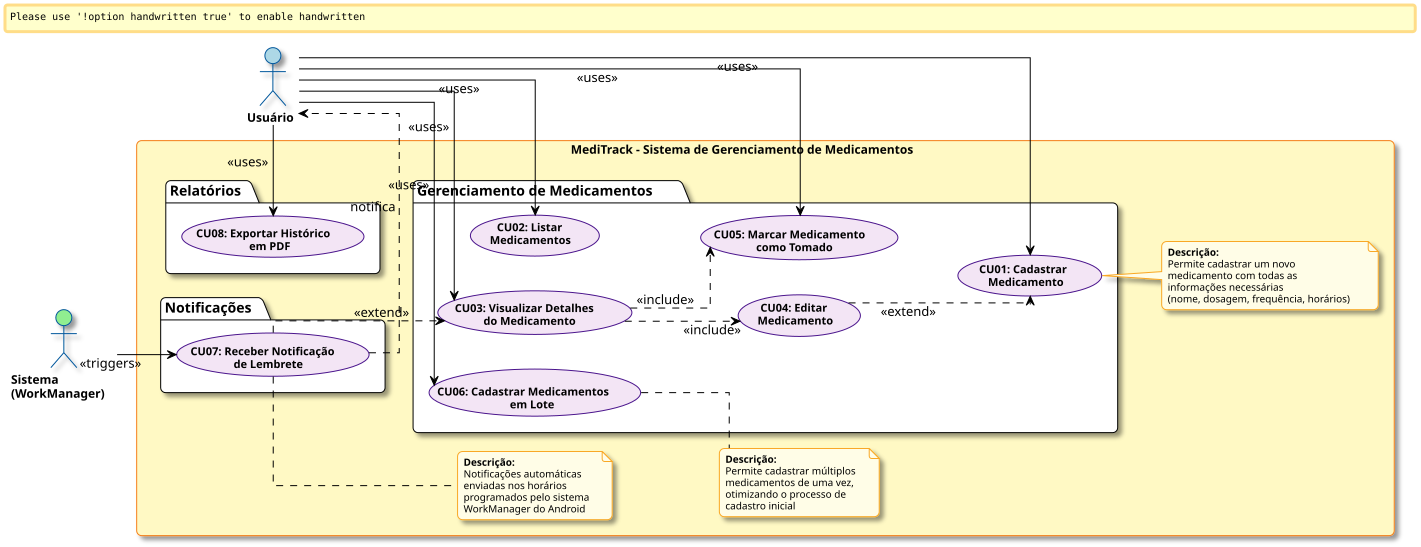
\includegraphics[width=\textwidth]{assets/diagrama_casos_uso.svg}
    \caption{Diagrama de Casos de Uso do Sistema MediTrack}
    \label{fig:diagrama_casos_uso}
\end{figure}

\subsubsection{Resumo dos Casos de Uso e Relacionamentos}

\begin{itemize}
    \item \textbf{Ator Principal:} Usuário
    \item \textbf{Casos de Uso:}
    \begin{itemize}
        \item CU01: Cadastrar Medicamento
        \item CU02: Listar Medicamentos
        \item CU03: Visualizar Detalhes do Medicamento
        \item CU04: Editar Medicamento
        \item CU05: Marcar Medicamento como Tomado
        \item CU06: Cadastrar Medicamentos em Lote
        \item CU07: Receber Notificação de Lembrete
        \item CU08: Exportar Histórico em PDF
    \end{itemize}
    \item \textbf{Relacionamentos:}
    \begin{itemize}
        \item CU03 inclui CU04 (para editar)
        \item CU03 inclui CU05 (para marcar como tomado)
        \item CU04 estende CU01 (comportamento similar de validação e salvamento)
        \item CU07 é iniciado pelo Sistema (WorkManager)
    \end{itemize}
\end{itemize}

\newpage

% ================================
% ENTREGA PARCIAL 3
% ================================
\section{MODELAGEM ESTRUTURAL E COMPORTAMENTAL}

\subsection{Diagrama de Classes}

\subsubsection{Descrição das Classes do Sistema MediTrack}

\textbf{Medication (Entidade)}

Classe que representa um medicamento no sistema. Possui informações sobre nome, dosagem, frequência, horários e status.

\textbf{Atributos:}
\begin{itemize}
    \item \texttt{id: Int} - Identificador único do medicamento
    \item \texttt{name: String} - Nome do medicamento
    \item \texttt{dosage: String} - Dosagem do medicamento
    \item \texttt{frequency: String} - Frequência de administração
    \item \texttt{schedule: String} - Horários de administração (ex: ``8h, 14h, 20h'')
    \item \texttt{status: String} - Status atual (Pendente, Tomado, Atrasado)
\end{itemize}

\textbf{Métodos:}
\begin{itemize}
    \item \texttt{isValid(): Boolean} - Valida se todos os campos obrigatórios foram preenchidos
\end{itemize}

\textbf{MedicationDao (Interface)}

Interface de acesso a dados (DAO) que define operações de persistência para medicamentos.

\textbf{Métodos:}
\begin{itemize}
    \item \texttt{insert(medication: Medication): suspend} - Insere um novo medicamento
    \item \texttt{update(medication: Medication): suspend} - Atualiza um medicamento existente
    \item \texttt{getAll(): Flow<List<Medication>>} - Obtém todos os medicamentos
    \item \texttt{getById(id: Int): suspend Medication?} - Obtém um medicamento por ID
\end{itemize}

\textbf{MedicationRepository (Interface)}

Interface do repositório que abstrai o acesso aos dados.

\textbf{Métodos:}
\begin{itemize}
    \item \texttt{insertMedication(medication: Medication): suspend}
    \item \texttt{updateMedication(medication: Medication): suspend}
    \item \texttt{getAllMedications(): Flow<List<Medication>>}
    \item \texttt{getMedicationById(id: Int): suspend Medication?}
\end{itemize}

\textbf{MedicationRepositoryImpl (Implementação)}

Implementação do repositório que utiliza o DAO para realizar operações.

\textbf{Relacionamentos:}
\begin{itemize}
    \item Utiliza \texttt{MedicationDao} para acesso aos dados
\end{itemize}

\textbf{MedicationDatabase}

Classe abstrata que representa o banco de dados Room.

\textbf{Métodos:}
\begin{itemize}
    \item \texttt{medicationDao(): MedicationDao} - Retorna a instância do DAO
\end{itemize}

\textbf{Relacionamentos:}
\begin{itemize}
    \item Contém \texttt{Medication} como entidade
\end{itemize}

\textbf{MedicationViewModel}

Classe que gerencia a lógica de apresentação seguindo o padrão MVVM.

\textbf{Atributos:}
\begin{itemize}
    \item \texttt{allMedications: Flow<List<Medication>>} - Fluxo reativo de todos os medicamentos
\end{itemize}

\textbf{Métodos:}
\begin{itemize}
    \item \texttt{insertMedication(medication: Medication)}
    \item \texttt{updateMedication(medication: Medication)}
    \item \texttt{markMedicationAsTaken(medication: Medication)}
    \item \texttt{getMedicationById(id: Int): Flow<Medication?>}
\end{itemize}

\textbf{Relacionamentos:}
\begin{itemize}
    \item Utiliza \texttt{MedicationRepository} para operações de dados
\end{itemize}

\textbf{NotificationScheduler}

Classe responsável por agendar notificações de lembretes.

\textbf{Métodos:}
\begin{itemize}
    \item \texttt{scheduleNotification(medication: Medication)} - Agenda notificações para um medicamento
\end{itemize}

\textbf{NotificationWorker}

Classe que executa o trabalho de envio de notificações usando WorkManager.

\textbf{Métodos:}
\begin{itemize}
    \item \texttt{doWork(): Result} - Método principal executado pelo WorkManager
    \item \texttt{showNotification(medicationName: String, medicationDosage: String): private} - Exibe a notificação
\end{itemize}

\textbf{PdfGenerator}

Classe responsável pela geração de relatórios em PDF.

\textbf{Métodos:}
\begin{itemize}
    \item \texttt{generateMedicationHistoryPdf(medications: List<Medication>): File?} - Gera PDF com histórico
\end{itemize}

\textbf{AppContainer (Interface)}

Interface que define o container de dependências.

\textbf{Atributos:}
\begin{itemize}
    \item \texttt{medicationDatabase: MedicationDatabase}
    \item \texttt{medicationRepository: MedicationRepository}
\end{itemize}

\textbf{AppDataContainer (Implementação)}

Implementação do container de dependências usando injeção manual.

\subsubsection{Relacionamentos entre Classes}

O diagrama de classes do sistema MediTrack apresenta os seguintes relacionamentos:

\begin{itemize}
    \item \texttt{MedicationRepositoryImpl} implementa a interface \texttt{MedicationRepository}
    \item \texttt{MedicationViewModel} utiliza \texttt{MedicationRepository} para operações de dados
    \item \texttt{MedicationDatabase} contém \texttt{MedicationDao} e armazena entidades \texttt{Medication}
    \item \texttt{NotificationScheduler} depende de \texttt{Medication} para agendar notificações
    \item \texttt{PdfGenerator} utiliza \texttt{Medication} para gerar relatórios
    \item \texttt{AppDataContainer} implementa \texttt{AppContainer} e cria as instâncias de \texttt{MedicationDatabase} e \texttt{MedicationRepositoryImpl}
\end{itemize}

\textbf{Código PlantUML do Diagrama de Classes:}

\begin{lstlisting}
@startuml Diagrama_Classes_MediTrack
!theme plain
skinparam backgroundColor #FFFFFF
skinparam handwritten false
skinparam monochrome false
skinparam shadowing true
skinparam roundcorner 10
skinparam linetype ortho

skinparam class {
    BackgroundColor #E3F2FD
    BorderColor #1976D2
    FontSize 11
    FontStyle bold
    AttributeFontSize 10
    AttributeFontStyle normal
    MethodFontSize 10
    MethodFontStyle italic
}

skinparam interface {
    BackgroundColor #F1F8E9
    BorderColor #558B2F
    FontSize 11
    FontStyle bold
    AttributeFontSize 10
    AttributeFontStyle normal
    MethodFontSize 10
    MethodFontStyle italic
}

skinparam abstract {
    BackgroundColor #FFF3E0
    BorderColor #E65100
    FontSize 11
    FontStyle bold
    AttributeFontSize 10
    AttributeFontStyle normal
    MethodFontSize 10
    MethodFontStyle italic
}

skinparam package {
    BackgroundColor #F5F5F5
    BorderColor #616161
}

skinparam arrow {
    Color #424242
    Thickness 2
}

package "Entidades" {
    class Medication {
        - id: Long
        - name: String
        - dosage: String
        - frequency: String
        - schedule: String
        - status: MedicationStatus
        - createdAt: LocalDateTime
        - updatedAt: LocalDateTime
        --
        + isValid(): Boolean
        + markAsTaken(): void
        + markAsDelayed(): void
    }
    
    enum MedicationStatus {
        PENDENTE
        TOMADO
        ATRASADO
    }
}

package "Persistência" {
    interface MedicationDao {
        + insert(medication: Medication): Long
        + update(medication: Medication): void
        + delete(id: Long): void
        + getAll(): Flow<List<Medication>>
        + getById(id: Long): Flow<Medication?>
        + getByStatus(status: MedicationStatus): Flow<List<Medication>>
    }
    
    abstract class MedicationDatabase {
        + medicationDao(): MedicationDao
        {abstract}
    }
    
    class AppDatabase {
        - INSTANCE: AppDatabase
        + medicationDao(): MedicationDao
        + getInstance(context: Context): AppDatabase
    }
}

package "Repositório" {
    interface MedicationRepository {
        + insertMedication(medication: Medication): Flow<Long>
        + updateMedication(medication: Medication): Flow<Unit>
        + deleteMedication(id: Long): Flow<Unit>
        + getAllMedications(): Flow<List<Medication>>
        + getMedicationById(id: Long): Flow<Medication?>
        + markMedicationAsTaken(id: Long): Flow<Unit>
    }
    
    class MedicationRepositoryImpl {
        - medicationDao: MedicationDao
        --
        + insertMedication(medication: Medication): Flow<Long>
        + updateMedication(medication: Medication): Flow<Unit>
        + deleteMedication(id: Long): Flow<Unit>
        + getAllMedications(): Flow<List<Medication>>
        + getMedicationById(id: Long): Flow<Medication?>
        + markMedicationAsTaken(id: Long): Flow<Unit>
    }
}

package "Apresentação" {
    class MedicationViewModel {
        - medicationRepository: MedicationRepository
        - _allMedications: MutableStateFlow<List<Medication>>
        - _selectedMedication: MutableStateFlow<Medication?>
        --
        + allMedications: StateFlow<List<Medication>>
        + selectedMedication: StateFlow<Medication?>
        + insertMedication(medication: Medication): Job
        + updateMedication(medication: Medication): Job
        + deleteMedication(id: Long): Job
        + markMedicationAsTaken(id: Long): Job
        + getMedicationById(id: Long): Job
    }
}

package "Notificações" {
    class NotificationScheduler {
        - context: Context
        - workManager: WorkManager
        --
        + scheduleNotification(medication: Medication): void
        + cancelNotification(medicationId: Long): void
        + rescheduleAllNotifications(): void
        - createWorkRequest(medication: Medication, time: LocalTime): PeriodicWorkRequest
    }
    
    class NotificationWorker {
        - applicationContext: Context
        - workerParams: WorkerParameters
        --
        + doWork(): Result
        - showNotification(medicationName: String, medicationDosage: String): void
        - createNotificationChannel(): void
    }
}

package "Relatórios" {
    class PdfGenerator {
        - context: Context
        - document: Document
        --
        + generateMedicationHistoryPdf(medications: List<Medication>): File?
        + generateMedicationReport(medication: Medication): File?
        - createDocumentHeader(): void
        - createMedicationTable(medications: List<Medication>): void
        - savePdfFile(document: Document): File?
    }
}

package "Injeção de Dependências" {
    interface AppContainer {
        + medicationDatabase: MedicationDatabase
        + medicationRepository: MedicationRepository
    }
    
    class AppDataContainer {
        - context: Context
        - _medicationDatabase: MedicationDatabase
        - _medicationRepository: MedicationRepository
        --
        + medicationDatabase: MedicationDatabase
        + medicationRepository: MedicationRepository
    }
}

' Relacionamentos - Entidades
Medication --> MedicationStatus : uses

' Relacionamentos - Persistência
AppDatabase --|> MedicationDatabase : extends
MedicationDatabase "1" *-- "0..*" Medication : stores
MedicationDatabase o-- MedicationDao : provides

' Relacionamentos - Repositório
MedicationRepositoryImpl ..|> MedicationRepository : implements
MedicationRepositoryImpl *-- MedicationDao : uses

' Relacionamentos - Apresentação
MedicationViewModel --> MedicationRepository : uses

' Relacionamentos - Notificações
NotificationScheduler --> Medication : uses
NotificationScheduler --> NotificationWorker : creates
NotificationWorker ..> Medication : uses

' Relacionamentos - Relatórios
PdfGenerator --> Medication : uses

' Relacionamentos - Injeção de Dependências
AppDataContainer ..|> AppContainer : implements
AppDataContainer *-- MedicationDatabase : creates
AppDataContainer *-- MedicationRepositoryImpl : creates

@enduml
\end{lstlisting}

\begin{figure}[H]
    \centering
    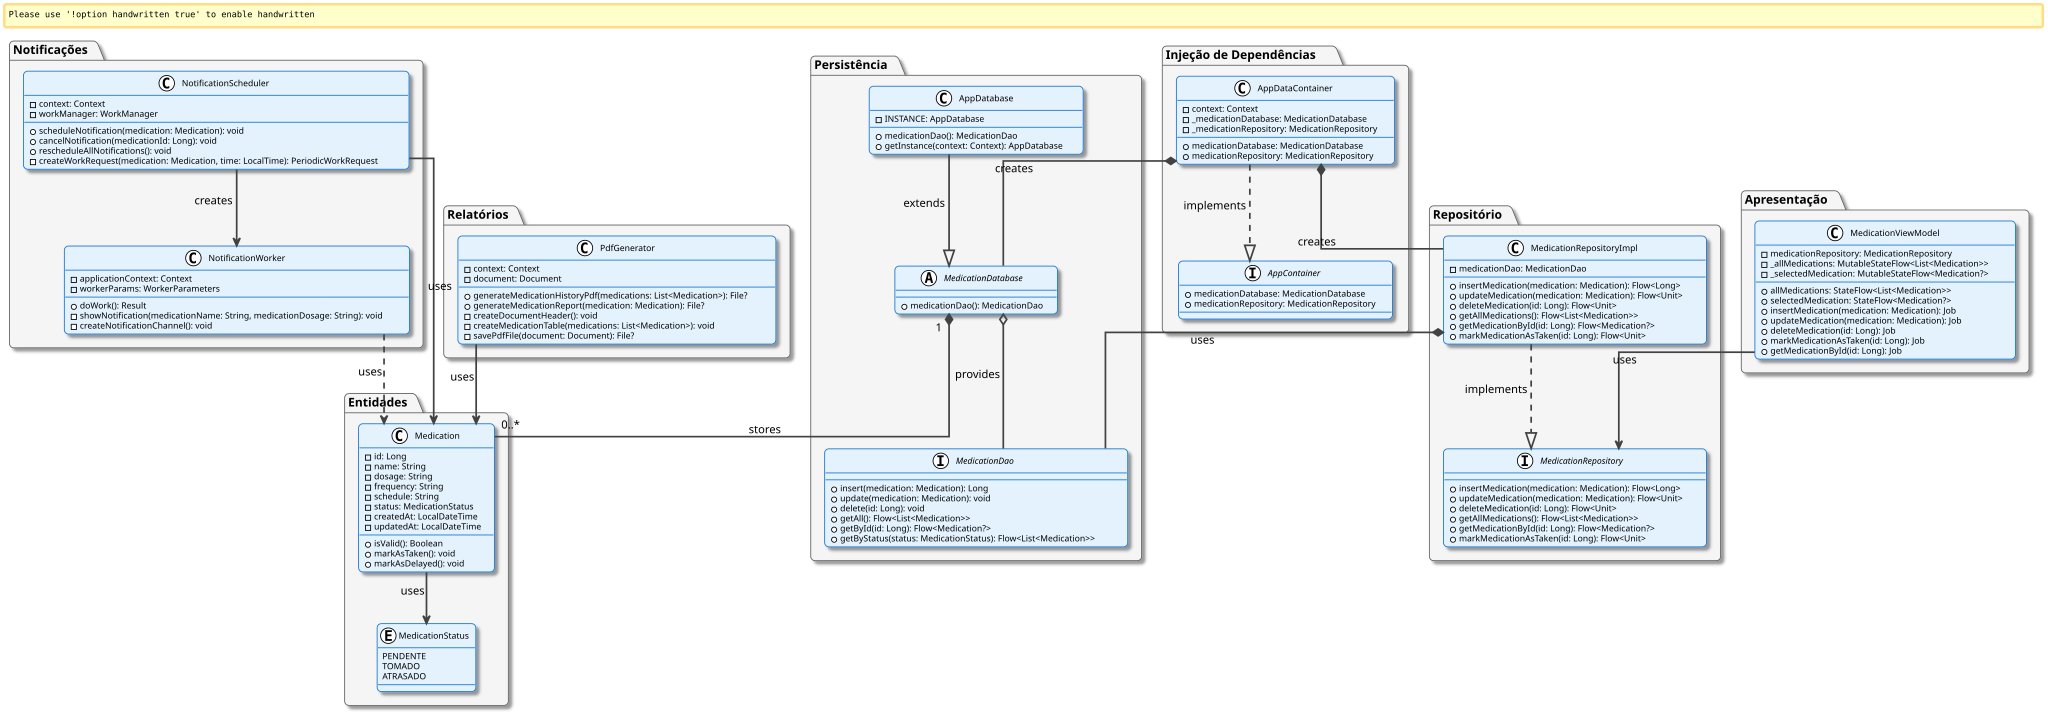
\includegraphics[width=\textwidth]{assets/diagrama_classes.svg}
    \caption{Diagrama de Classes do Sistema MediTrack}
    \label{fig:diagrama_classes}
\end{figure}

\subsection{Diagrama de Atividades}

\subsubsection{Processo: Cadastrar Medicamento e Agendar Notificação}

Este processo envolve desde o preenchimento do formulário pelo usuário até o agendamento das notificações pelo sistema, sendo um processo crítico para o funcionamento do aplicativo.

\subsubsection{Fluxo de Atividades}

\begin{enumerate}
    \item Usuário acessa formulário de cadastro
    \item Sistema exibe campos do formulário
    \item Usuário preenche informações (nome, dosagem, frequência, horário)
    \item Sistema valida campos obrigatórios
    \item Se inválido: exibe mensagem de erro e retorna ao passo 3
    \item Se válido: cria objeto Medication
    \item Sistema salva medicamento no banco de dados
    \item Sistema agenda notificações para os horários informados
    \item Sistema parse do horário (ex: ``8h, 14h, 20h'')
    \item Para cada horário:
    \begin{itemize}
        \item Sistema calcula delay até o horário
        \item Sistema cria PeriodicWorkRequest
        \item Sistema agenda notificação com WorkManager
    \end{itemize}
    \item Sistema retorna à tela de lista
    \item Fim do processo
\end{enumerate}


\textbf{Código PlantUML do Diagrama de Atividades:}

\begin{lstlisting}
@startuml Diagrama_Atividades_Cadastrar_Medicamento
!theme plain
skinparam backgroundColor #FFFFFF
skinparam handwritten false
skinparam monochrome false
skinparam shadowing true
skinparam roundcorner 10
skinparam activity {
    BackgroundColor #E1F5FE
    BorderColor #01579B
    FontSize 11
    FontStyle bold
}

skinparam partition {
    BackgroundColor #F3E5F5
    BorderColor #4A148C
    FontSize 11
    FontStyle bold
}

skinparam note {
    BackgroundColor #FFFDE7
    BorderColor #F9A825
    FontSize 10
}

start

partition "Interface do Usuário" {
    :Usuário acessa tela de\ncadastro de medicamento;
    :Sistema exibe formulário\ncom campos obrigatórios;
    note right
        Campos: Nome, Dosagem,
        Frequência, Horários
    end note
}

partition "Validação" {
    :Usuário preenche informações\ndo medicamento;
    :Sistema valida campos obrigatórios;
    
    if (Todos os campos válidos?) then (não)
        :Sistema exibe mensagens\nde erro específicas;
        :Usuário corrige informações;
        :Sistema valida campos obrigatórios;
    endif
}

partition "Persistência" {
    :Sistema cria objeto Medication\ncom dados informados;
    :Sistema define status inicial\ncomo PENDENTE;
    :Sistema salva medicamento\nno banco de dados;
    
    if (Medicamento salvo com sucesso?) then (não)
        :Sistema exibe mensagem\nde erro ao salvar;
        stop
    endif
}

partition "Agendamento de Notificações" {
    :Sistema faz parse do campo\nschedule (ex: "8h, 14h, 20h");
    
    :Sistema extrai lista\nde horários;
    
    while (Há mais horários para processar?) is (sim)
        :Sistema calcula delay\ndo horário atual até o horário\nda primeira dose;
        
        :Sistema cria PeriodicWorkRequest\ncom frequência diária;
        
        :Sistema agenda notificação\nusando WorkManager;
        
        note right
            WorkManager garante
            que a notificação será
            exibida mesmo se o app
            estiver em background
        end note
    endwhile (não há mais horários)
    
    :Sistema registra todas as\nnotificações agendadas;
}

partition "Feedback ao Usuário" {
    :Sistema atualiza lista\nde medicamentos;
    :Sistema exibe mensagem\nde sucesso;
    :Sistema retorna à tela\nde listagem;
    stop
}

@enduml
\end{lstlisting}

\begin{figure}[H]
    \centering
    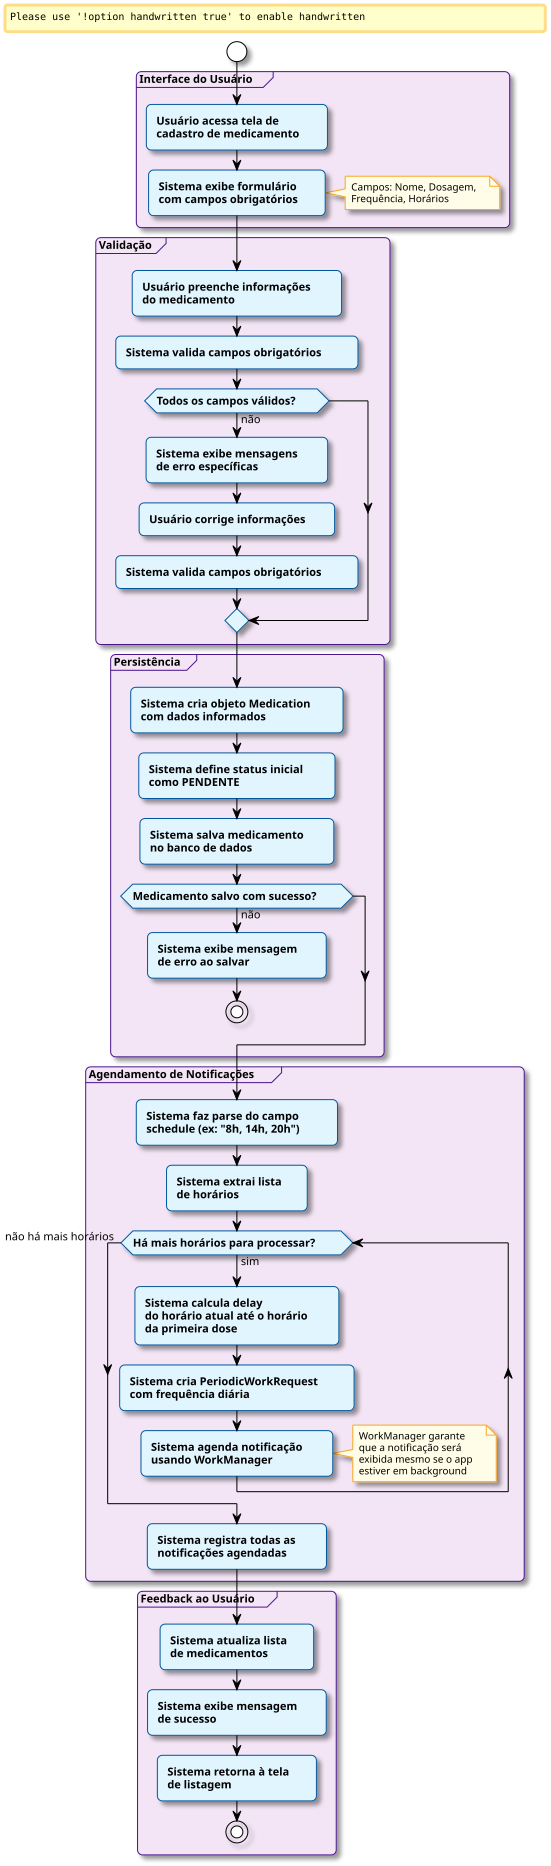
\includegraphics[width=\textwidth]{assets/diagrama_atividades.svg}
    \caption{Diagrama de Atividades - Cadastrar Medicamento e Agendar Notificação}
    \label{fig:diagrama_atividades}
\end{figure}

\subsection{Diagrama de Sequência}

\subsubsection{Processo: Marcar Medicamento como Tomado}

Este processo mostra a sequência de chamadas entre os componentes do sistema quando o usuário marca um medicamento como tomado.

\subsubsection{Participantes}

\begin{itemize}
    \item \textbf{Usuário:} Ator que interage com o sistema
    \item \textbf{MedicationDetailScreen:} Tela de detalhes do medicamento
    \item \textbf{MedicationViewModel:} ViewModel que gerencia a lógica
    \item \textbf{MedicationRepository:} Camada de repositório
    \item \textbf{MedicationDao:} Camada de acesso a dados
    \item \textbf{MedicationDatabase:} Banco de dados Room
\end{itemize}

\subsubsection{Fluxo de Sequência}

\begin{enumerate}
    \item Usuário clica em ``Marcar como Tomado''
    \item MedicationDetailScreen chama \texttt{markMedicationAsTaken()} no ViewModel
    \item MedicationViewModel cria cópia do medicamento com status ``Tomado''
    \item MedicationViewModel chama \texttt{updateMedication()} no Repository
    \item MedicationRepository chama \texttt{update()} no DAO
    \item MedicationDao executa UPDATE no Database
    \item MedicationDatabase persiste a atualização
    \item O fluxo reativo (\texttt{Flow}) notifica os observadores
    \item MedicationViewModel atualiza o estado
    \item MedicationDetailScreen atualiza a interface
    \item Botão ``Marcar como Tomado'' desaparece da tela
\end{enumerate}


\textbf{Código PlantUML do Diagrama de Sequência:}

\begin{lstlisting}
@startuml Diagrama_Sequencia_Marcar_Como_Tomado
!theme plain
skinparam backgroundColor #FFFFFF
skinparam handwritten false
skinparam monochrome false
skinparam shadowing true
skinparam roundcorner 10
skinparam maxMessageSize 60
skinparam linetype ortho

skinparam actor {
    BackgroundColor #E1F5FE
    BorderColor #01579B
    FontSize 12
    FontStyle bold
}

skinparam participant {
    BackgroundColor #F3E5F5
    BorderColor #4A148C
    FontSize 11
    FontStyle bold
}

skinparam database {
    BackgroundColor #E8F5E9
    BorderColor #2E7D32
    FontSize 11
    FontStyle bold
}

skinparam arrow {
    Color #424242
    Thickness 2
}

skinparam note {
    BackgroundColor #FFFDE7
    BorderColor #F9A825
    FontSize 10
}

actor "Usuário" as Usuario #LightBlue
participant "MedicationDetailScreen" as Screen #LightCoral
participant "MedicationViewModel" as ViewModel #LightGreen
participant "MedicationRepository" as Repository #LightYellow
participant "MedicationDao" as Dao #LightPink
database "Room Database" as Database #LightGreen

Usuario -> Screen: 1. Clica no botão\n"Marcar como Tomado"
activate Screen

Screen -> Screen: 2. Valida se medicamento\nnão está já marcado

alt Medicamento já está marcado
    Screen --> Usuario: Exibe mensagem:\n"Medicamento já foi tomado"
    
else Medicamento não está marcado
    Screen -> ViewModel: 3. markMedicationAsTaken(\nmedicationId: Long)
    activate ViewModel
    
    ViewModel -> ViewModel: 4. Cria cópia do medicamento\ncom status = TOMADO
    
    ViewModel -> ViewModel: 5. Atualiza updatedAt\ncom timestamp atual
    
    ViewModel -> Repository: 6. updateMedication(\nmedication: Medication)
    activate Repository
    
    Repository -> Repository: 7. Valida dados\ndo medicamento
    
    Repository -> Dao: 8. update(medication: Medication)
    activate Dao
    
    Dao -> Database: 9. UPDATE medications\nSET status = 'TOMADO',\nupdatedAt = NOW()\nWHERE id = ?
    activate Database
    
    Database --> Dao: 10. Retorna número de\nlinhas afetadas
    deactivate Database
    
    alt Atualização bem-sucedida
        Dao --> Repository: 11. Sucesso (rows > 0)
        deactivate Dao
        
        Repository --> ViewModel: 12. Flow emite\nmedication atualizado
        deactivate Repository
        
        note right of ViewModel
            O Flow reativo notifica
            automaticamente todos os
            observadores (StateFlow)
            sobre a mudança de estado
        end note
        
        ViewModel -> ViewModel: 13. Atualiza StateFlow\nallMedications
        
        ViewModel --> Screen: 14. Estado atualizado\nvia StateFlow
        deactivate ViewModel
        
        Screen -> Screen: 15. Atualiza UI com\nnovo estado
        
        Screen -> Screen: 16. Remove botão\n"Marcar como Tomado"
        
        Screen -> Screen: 17. Exibe indicador\n"Medicamento Tomado"
        
        Screen --> Usuario: 18. Interface atualizada\ncom feedback visual
        
    else Erro na atualização
        Dao --> Repository: 11. Erro (rows = 0)
        deactivate Dao
        
        Repository --> ViewModel: 12. Flow emite erro
        deactivate Repository
        
        ViewModel --> Screen: 13. Erro ao atualizar
        deactivate ViewModel
        
        Screen --> Usuario: 14. Exibe mensagem de erro
        
    end
    
end

deactivate Screen

@enduml
\end{lstlisting}

\begin{figure}[H]
    \centering
    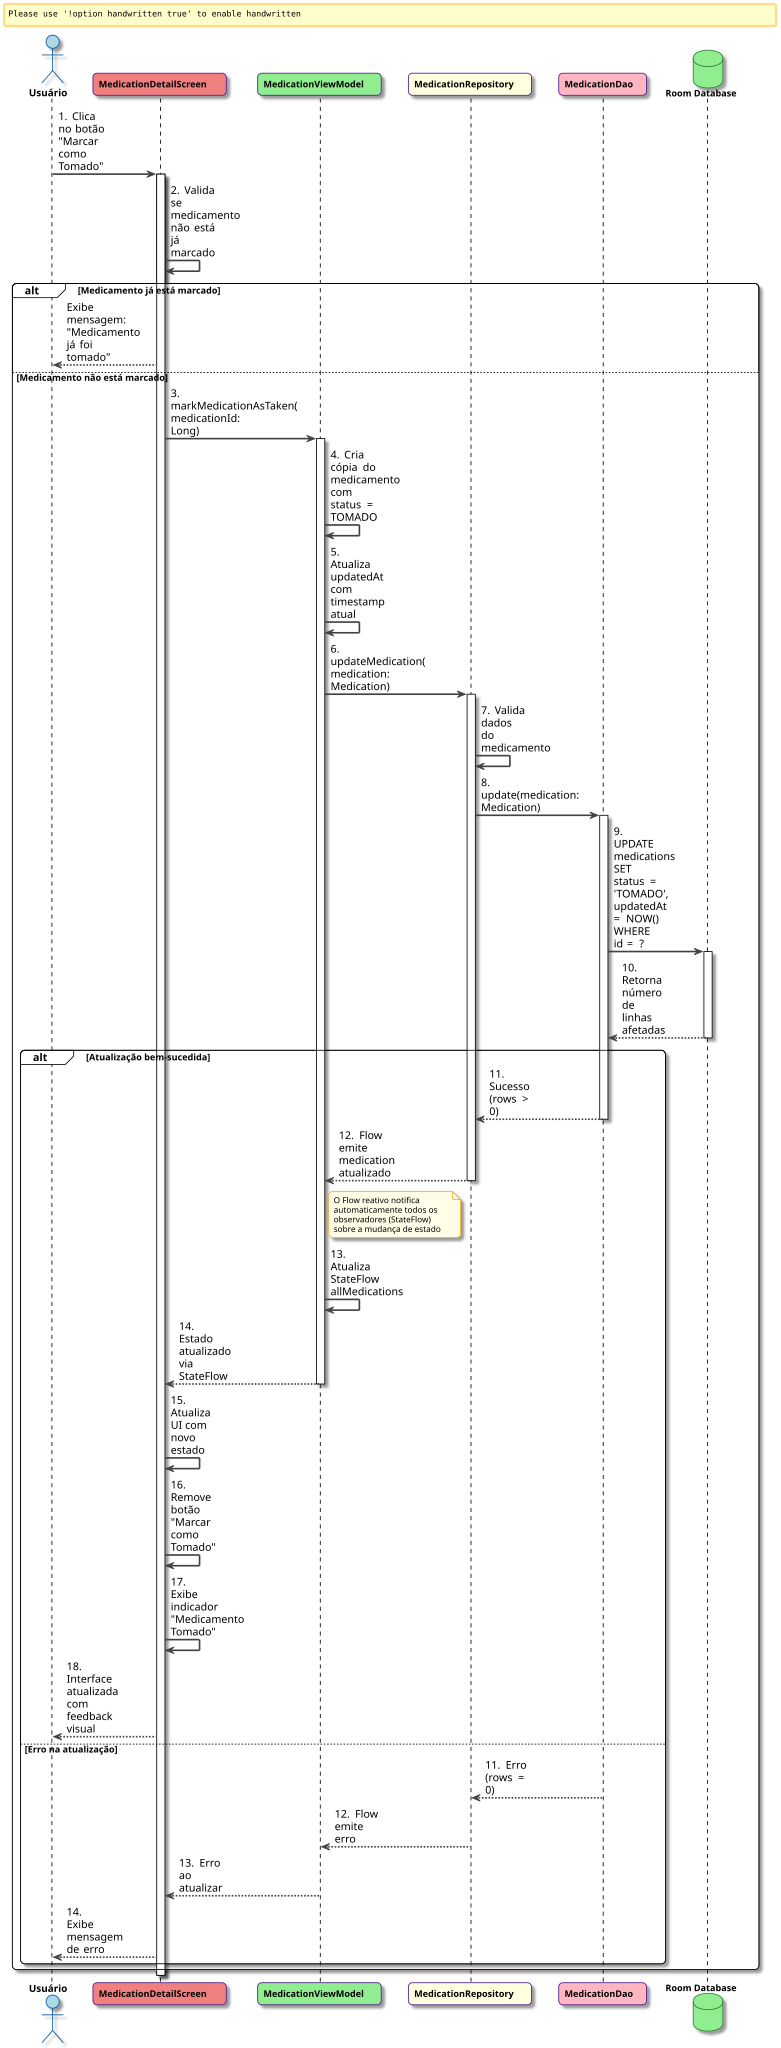
\includegraphics[width=\textwidth]{assets/diagrama_sequencia.svg}
    \caption{Diagrama de Sequência - Marcar Medicamento como Tomado}
    \label{fig:diagrama_sequencia}
\end{figure}

\subsection{Diagrama de Estados}

\subsubsection{Estados do Medicamento no Sistema MediTrack}

\begin{enumerate}
    \item \textbf{Pendente:} Estado inicial quando o medicamento é cadastrado
    \item \textbf{Tomado:} Estado quando o usuário marca o medicamento como tomado
    \item \textbf{Atrasado:} Estado quando o horário passou e o medicamento não foi marcado como tomado (futuro)
\end{enumerate}

\subsubsection{Transições}

\begin{itemize}
    \item \textbf{Cadastrar:} [Estado inicial] $\rightarrow$ Pendente
    \item \textbf{Marcar como Tomado:} Pendente $\rightarrow$ Tomado
    \item \textbf{Marcar como Tomado:} Atrasado $\rightarrow$ Tomado
    \item \textbf{Horário Passou (sistema):} Pendente $\rightarrow$ Atrasado (lógica futura)
\end{itemize}


\textbf{Código PlantUML do Diagrama de Estados:}

\begin{lstlisting}
@startuml Diagrama_Estados_Medicamento
!theme plain
skinparam backgroundColor #FFFFFF
skinparam handwritten false
skinparam monochrome false
skinparam shadowing true
skinparam roundcorner 10

skinparam state {
    BackgroundColor #E3F2FD
    BorderColor #1976D2
    FontSize 11
    FontStyle bold
}

skinparam arrow {
    Color #424242
    Thickness 2
}

skinparam note {
    BackgroundColor #FFFDE7
    BorderColor #F9A825
    FontSize 10
}

[*] --> Pendente : Cadastrar medicamento

state Pendente {
    state "Medicamento cadastrado" as P1
    state "Aguardando horário\nda primeira dose" as P2
    
    P1 --> P2 : Horário agendado
}

state Atrasado {
    state "Horário da dose passou" as A1
    state "Medicamento não tomado" as A2
    state "Sistema detecta atraso" as A3
    
    A1 --> A2 : Horário passou
    A2 --> A3 : Sistema verifica status
}

state Tomado {
    state "Usuário marca como tomado" as T1
    state "Registrado data/hora" as T2
    state "Status finalizado" as T3
    
    T1 --> T2 : Confirmação
    T2 --> T3 : Persistido no BD
}

Pendente --> Tomado : marcarComoTomado()\n[usuário confirma]
Pendente --> Atrasado : verificarHorario()\n[horário passou && status = PENDENTE]
Atrasado --> Tomado : marcarComoTomado()\n[usuário confirma]

note right of Pendente
    <b>Estado Inicial</b>
    Quando o medicamento é
    cadastrado, ele inicia
    no estado PENDENTE.
    O sistema aguarda o
    horário programado.
end note

note right of Atrasado
    <b>Estado de Atraso</b>
    O sistema verifica
    periodicamente se o
    horário passou sem
    o medicamento ser tomado.
    Pode ser marcado como
    tomado mesmo estando atrasado.
end note

note right of Tomado
    <b>Estado Final</b>
    Quando o usuário marca
    como tomado, o sistema
    registra a data e hora
    exata da confirmação.
    Este é um estado terminal
    para aquela dose específica.
end note

@enduml
\end{lstlisting}

\begin{figure}[H]
    \centering
    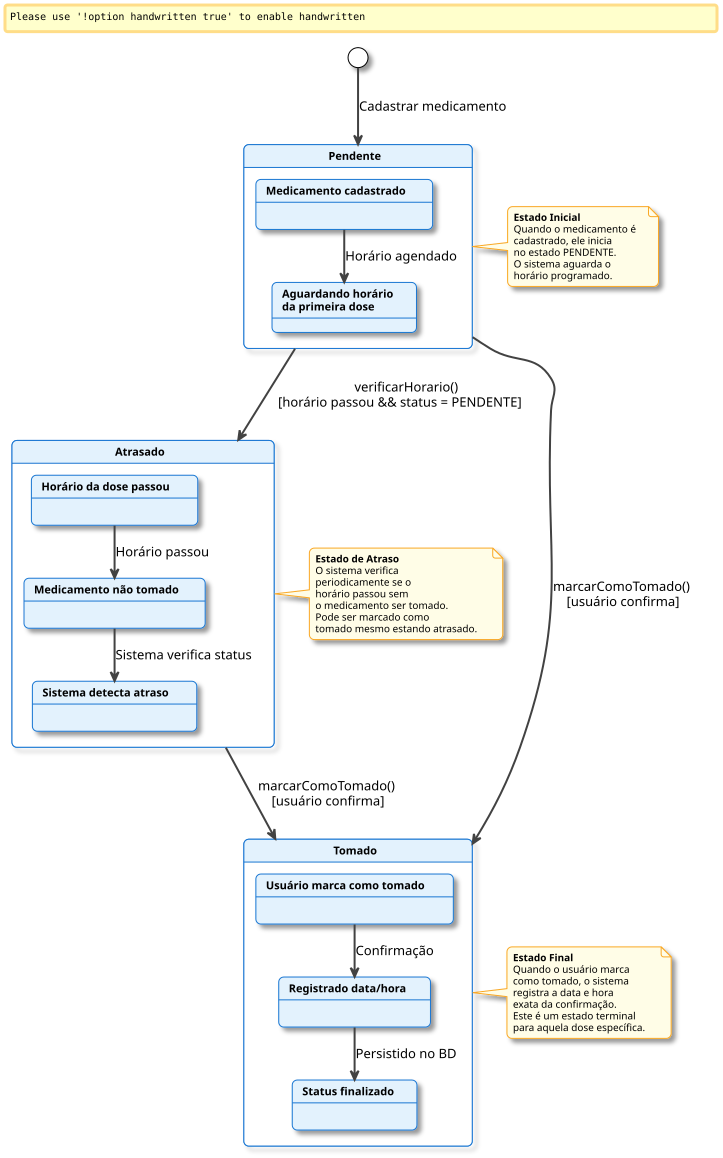
\includegraphics[width=\textwidth]{assets/diagrama_estados.svg}
    \caption{Diagrama de Estados do Medicamento}
    \label{fig:diagrama_estados}
\end{figure}

\subsection{Aplicação de Conceitos OOP}

\subsubsection{Encapsulamento}

\begin{itemize}
    \item Todas as classes encapsulam seus dados e comportamentos
    \item Atributos privados são acessados através de métodos públicos
    \item Exemplo: \texttt{Medication.isValid()} encapsula a lógica de validação
\end{itemize}

\subsubsection{Herança/Implementação}

\begin{itemize}
    \item \texttt{MedicationRepositoryImpl} implementa a interface \texttt{MedicationRepository}
    \item \texttt{AppDataContainer} implementa a interface \texttt{AppContainer}
    \item \texttt{NotificationWorker} herda de \texttt{Worker} (Android WorkManager)
\end{itemize}

\subsubsection{Polimorfismo}

\begin{itemize}
    \item O uso de interfaces permite polimorfismo
    \item \texttt{MedicationRepository} pode ser substituído por diferentes implementações
    \item Diferentes tipos de \texttt{Worker} podem ser usados para diferentes tarefas
\end{itemize}

\subsubsection{Abstração}

\begin{itemize}
    \item Interfaces (\texttt{MedicationRepository}, \texttt{MedicationDao}) abstraem implementações
    \item A camada de ViewModel abstrai a lógica de negócio da UI
\end{itemize}

\subsubsection{Relacionamentos}

\begin{itemize}
    \item \textbf{Associação:} \texttt{MedicationViewModel} $\rightarrow$ \texttt{MedicationRepository}
    \item \textbf{Agregação:} \texttt{MedicationDatabase} $\rightarrow$ \texttt{MedicationDao}
    \item \textbf{Composição:} \texttt{MedicationDatabase} compõe \texttt{Medication} (persistência)
    \item \textbf{Dependência:} \texttt{NotificationScheduler} depende de \texttt{Medication}
\end{itemize}

\newpage

% ================================
% ENTREGA PARCIAL 4
% ================================
\section{GERENCIAMENTO E RASTREABILIDADE DOS REQUISITOS}

\subsection{Ferramenta de Gerenciamento Escolhida}

\subsubsection{Jira}

Foi escolhida a ferramenta \textbf{Jira} para o gerenciamento do projeto devido às seguintes vantagens:

\begin{itemize}
    \item \textbf{Profissional:} Ferramenta amplamente utilizada na indústria de software
    \item \textbf{Rastreabilidade:} Permite rastreamento completo de requisitos através de issues, epics e links
    \item \textbf{Hierárquica:} Suporta estrutura hierárquica (Epic $\rightarrow$ Story $\rightarrow$ Task $\rightarrow$ Sub-task)
    \item \textbf{Relacionamentos:} Possibilita criação de relacionamentos entre issues (relates to, blocks, etc.)
    \item \textbf{Relatórios:} Oferece relatórios e métricas de rastreabilidade
    \item \textbf{Labels e Componentes:} Permite categorização através de labels e componentes
    \item \textbf{Importação CSV:} Suporta importação em massa via arquivo CSV
\end{itemize}

\subsubsection{Link do Projeto}

\textbf{Link do Projeto Jira:} [AQUI DEVE SER INSERIDO O LINK DO PROJETO JIRA]

Exemplo de estrutura:
\begin{itemize}
    \item \texttt{https://seu-workspace.atlassian.net/jira/software/projects/MED/board}
    \item \texttt{https://seu-workspace.atlassian.net/browse/MED}
\end{itemize}

\subsection{Estrutura do Projeto no Jira}

\subsubsection{Organização do Projeto}

O projeto foi organizado com as seguintes \textbf{Issue Types}:

\begin{enumerate}
    \item \textbf{Epics (Épicos):}
    \begin{itemize}
        \item Entrega Parcial 1: Definição do Problema e Elicitação
        \item Entrega Parcial 2: Casos de Uso
        \item Entrega Parcial 3: Diagramas UML
        \item Entrega Parcial 4: Gerenciamento e Rastreabilidade
        \item Entrega Final: Relatório e Apresentação
    \end{itemize}
    
    \item \textbf{Stories (Histórias):}
    \begin{itemize}
        \item Requisitos funcionais (RF01 a RF10)
    \end{itemize}
    
    \item \textbf{Tasks (Tarefas):}
    \begin{itemize}
        \item Requisitos não funcionais (RNF01 a RNF08)
        \item Casos de Uso (CU01 a CU08)
        \item Diagramas UML
    \end{itemize}
    
    \item \textbf{Status:}
    \begin{itemize}
        \item To Do
        \item In Progress
        \item Done
    \end{itemize}
\end{enumerate}

\subsection{Rastreabilidade dos Requisitos}

\subsubsection{Matriz de Rastreabilidade}

A rastreabilidade foi estabelecida conectando cada requisito aos seus artefatos relacionados. A seguir está a matriz completa:

\textbf{Requisitos Funcionais}

\begin{longtable}{|p{2cm}|p{4cm}|p{3cm}|p{3cm}|p{4cm}|}
\hline
\textbf{ID} & \textbf{Requisito} & \textbf{Casos de Uso} & \textbf{Diagramas UML} & \textbf{Implementação} \\
\hline
\endfirsthead
\hline
\textbf{ID} & \textbf{Requisito} & \textbf{Casos de Uso} & \textbf{Diagramas UML} & \textbf{Implementação} \\
\hline
\endhead
RF01 & Cadastrar Medicamento & CU01 & Classes, Atividades & \texttt{AddEditMedicationScreen.kt} \\
\hline
RF02 & Listar Medicamentos & CU02 & Classes & \texttt{MedicationListScreen.kt} \\
\hline
RF03 & Visualizar Detalhes & CU03 & Classes, Sequência & \texttt{MedicationDetailScreen.kt} \\
\hline
RF04 & Editar Medicamento & CU04 & Classes, Atividades & \texttt{AddEditMedicationScreen.kt} \\
\hline
RF05 & Marcar como Tomado & CU05 & Classes, Sequência, Estados & \texttt{MedicationViewModel.kt} \\
\hline
RF06 & Cadastro em Lote & CU06 & Classes & \texttt{BulkAddMedicationScreen.kt} \\
\hline
RF07 & Notificações de Lembrete & CU07 & Classes, Atividades & \texttt{NotificationScheduler.kt}, \texttt{NotificationWorker.kt} \\
\hline
RF08 & Histórico de Uso & CU02, CU03 & Classes & \texttt{MedicationListScreen.kt} \\
\hline
RF09 & Exportar Histórico PDF & CU08 & Classes & \texttt{PdfGenerator.kt} \\
\hline
RF10 & Validar Dados & CU01, CU04 & Classes & \texttt{Medication.kt} \\
\hline
\end{longtable}

\textbf{Requisitos Não Funcionais}

\begin{longtable}{|p{2cm}|p{4cm}|p{4cm}|p{4cm}|}
\hline
\textbf{ID} & \textbf{Requisito} & \textbf{Artefatos Relacionados} & \textbf{Implementação} \\
\hline
\endfirsthead
\hline
\textbf{ID} & \textbf{Requisito} & \textbf{Artefatos Relacionados} & \textbf{Implementação} \\
\hline
\endhead
RNF01 & Performance & Diagrama de Classes & Arquitetura MVVM \\
\hline
RNF02 & Usabilidade & Casos de Uso & Interface Jetpack Compose \\
\hline
RNF03 & Confiabilidade & Diagrama de Classes & Room Database \\
\hline
RNF04 & Disponibilidade & Diagrama de Classes & Armazenamento local \\
\hline
RNF05 & Escalabilidade & Diagrama de Classes & Room Database otimizado \\
\hline
RNF06 & Segurança & Diagrama de Classes & Armazenamento local \\
\hline
RNF07 & Compatibilidade & Documentação & \texttt{build.gradle.kts} \\
\hline
RNF08 & Notificações & Diagrama de Atividades & WorkManager \\
\hline
\end{longtable}

\subsubsection{Cadastro e Gerenciamento dos Requisitos}

Os requisitos foram cadastrados e gerenciados no Jira através das seguintes etapas:

\textbf{1. Importação Inicial:}
\begin{itemize}
    \item Todos os requisitos foram importados em massa através de um arquivo CSV (\texttt{jira\_import.csv})
    \item O arquivo CSV continha 41 issues no total, incluindo:
    \begin{itemize}
        \item 10 Requisitos Funcionais (RF01-RF10) como Stories
        \item 8 Requisitos Não Funcionais (RNF01-RNF08) como Tasks
        \item 8 Casos de Uso (CU01-CU08) como Tasks
        \item 5 Entregas Parciais como Epics
        \item 5 Diagramas UML como Tasks
        \item 5 Issues adicionais de gerenciamento
    \end{itemize}
    \item Cada issue foi configurada com Summary, Issue Type, Description, Priority, Status e Labels apropriados
\end{itemize}

\textbf{2. Estruturação Hierárquica:}
\begin{itemize}
    \item \textbf{Epics:} Organizados por Entregas Parciais, servindo como containers principais
    \item \textbf{Stories:} Requisitos Funcionais vinculados aos seus respectivos Epics
    \item \textbf{Tasks:} Requisitos Não Funcionais, Casos de Uso e Diagramas vinculados aos Epics correspondentes
    \item \textbf{Sub-tasks:} Criadas para rastrear o progresso de cada artefato relacionado
\end{itemize}

\textbf{3. Organização por Labels:}
\begin{itemize}
    \item Labels utilizados para categorização: ``Requisito Funcional'', ``Requisito Não Funcional'', ``Caso de Uso'', ``Diagrama UML'', ``Entrega Parcial'', ``Alta Prioridade'', ``Média Prioridade'', etc.
    \item Labels facilitam filtragem e visualização de issues relacionadas
\end{itemize}

\textbf{4. Descrições Detalhadas:}
\begin{itemize}
    \item Cada issue contém descrição completa incluindo:
    \begin{itemize}
        \item Tipo de requisito (Funcional ou Não Funcional)
        \item Prioridade (Alta, Média ou Baixa)
        \item Fonte da elicitação (Entrevista, Questionário, Observação)
        \item Descrição detalhada do requisito
        \item Lista de artefatos relacionados (Casos de Uso, Diagramas, Implementação)
    \end{itemize}
\end{itemize}

\subsubsection{Rastreabilidade no Jira}

A rastreabilidade foi estabelecida e mantida no Jira através de:

\begin{enumerate}
    \item \textbf{Issue Links:} Cada issue de requisito possui links para:
    \begin{itemize}
        \item Issues de casos de uso relacionados (usando ``Relates to'')
        \item Issues de diagramas UML relacionados
        \item Issues de implementação relacionadas
    \end{itemize}
    
    \item \textbf{Epic Links:} Hierarquia organizada através de Epic Links:
    \begin{itemize}
        \item Epics representam Entregas Parciais
        \item Stories representam Requisitos Funcionais vinculados aos Epics
        \item Tasks representam Requisitos Não Funcionais e outros artefatos vinculados aos Epics
    \end{itemize}
    
    \item \textbf{Description:} Cada issue contém links diretos para:
    \begin{itemize}
        \item Documentos de entrega parcial (arquivos Markdown)
        \item Diagramas UML (arquivos .puml ou imagens)
        \item Código fonte (quando disponível em repositório Git)
    \end{itemize}
    
    \item \textbf{Sub-tasks:} Permitem rastrear o progresso de cada artefato relacionado ao requisito
    
    \item \textbf{Labels:} Categorização e filtragem de issues para facilitar a visualização da rastreabilidade
\end{enumerate}

\subsection{Planejamento de Entregas}

\subsubsection{Backlog de Tarefas}

O backlog foi organizado seguindo a ordem das entregas parciais:

\textbf{Sprint 1: Elicitação de Requisitos}
\begin{itemize}
    \item[$\checkmark$] Escolher sistema a ser modelado
    \item[$\checkmark$] Aplicar técnicas de elicitação (Entrevista, Questionário, Observação)
    \item[$\checkmark$] Documentar requisitos funcionais
    \item[$\checkmark$] Documentar requisitos não funcionais
    \item[$\checkmark$] Elaborar Entrega Parcial 1
\end{itemize}

\textbf{Sprint 2: Modelagem de Casos de Uso}
\begin{itemize}
    \item[$\checkmark$] Criar casos de uso detalhados
    \item[$\checkmark$] Elaborar diagrama de casos de uso
    \item[$\checkmark$] Revisar casos de uso
    \item[$\checkmark$] Elaborar Entrega Parcial 2
\end{itemize}

\textbf{Sprint 3: Diagramas UML Estruturais e Comportamentais}
\begin{itemize}
    \item[$\checkmark$] Criar diagrama de classes
    \item[$\checkmark$] Criar diagrama de atividades
    \item[$\checkmark$] Criar diagrama de sequência
    \item[$\checkmark$] Criar diagrama de estados
    \item[$\checkmark$] Elaborar Entrega Parcial 3
\end{itemize}

\textbf{Sprint 4: Gerenciamento e Rastreabilidade}
\begin{itemize}
    \item[$\checkmark$] Configurar ferramenta de gerenciamento (Jira)
    \item[$\checkmark$] Cadastrar todos os requisitos via importação CSV
    \item[$\checkmark$] Estabelecer rastreabilidade
    \item[$\checkmark$] Criar matriz de rastreabilidade
    \item[$\checkmark$] Elaborar Entrega Parcial 4
\end{itemize}

\textbf{Sprint 5: Relatório Final}
\begin{itemize}
    \item[ ] Consolidar todas as entregas parciais
    \item[ ] Elaborar relatório final
    \item[ ] Criar apresentação (slides)
    \item[ ] Revisar documentação completa
    \item[ ] Preparar apresentação oral
\end{itemize}

\subsubsection{Timeline do Projeto}

\begin{longtable}{|p{5cm}|p{4cm}|p{3cm}|}
\hline
\textbf{Entrega} & \textbf{Data Limite} & \textbf{Status} \\
\hline
\endfirsthead
\hline
\textbf{Entrega} & \textbf{Data Limite} & \textbf{Status} \\
\hline
\endhead
Entrega Parcial 1 & [Data] & Concluído \\
\hline
Entrega Parcial 2 & [Data] & Concluído \\
\hline
Entrega Parcial 3 & [Data] & Concluído \\
\hline
Entrega Parcial 4 & [Data] & Concluído \\
\hline
Entrega Final & 10/02/2026 & Em andamento \\
\hline
\end{longtable}

\subsection{Métricas de Rastreabilidade}

\subsubsection{Cobertura de Rastreabilidade}

\begin{itemize}
    \item \textbf{Total de Requisitos:} 18 (10 funcionais + 8 não funcionais)
    \item \textbf{Requisitos Rastreados:} 18 (100\%)
    \item \textbf{Artefatos Criados:}
    \begin{itemize}
        \item 8 Casos de Uso
        \item 4 Diagramas UML (Classes, Atividades, Sequência, Estados)
        \item 1 Diagrama de Casos de Uso
    \end{itemize}
\end{itemize}

\subsubsection{Status dos Requisitos}

\begin{itemize}
    \item \textbf{Implementados:} 18/18 (100\%)
    \item \textbf{Documentados:} 18/18 (100\%)
    \item \textbf{Rastreados:} 18/18 (100\%)
\end{itemize}

\subsection{Conclusão}

O gerenciamento de requisitos através do Jira permitiu:

\begin{enumerate}
    \item \textbf{Organização:} Todos os requisitos e artefatos estão organizados e acessíveis
    \item \textbf{Rastreabilidade:} É possível rastrear cada requisito desde sua origem até a implementação
    \item \textbf{Colaboração:} A dupla pode trabalhar de forma colaborativa e acompanhar o progresso
    \item \textbf{Controle:} O checklist permite verificar se todos os artefatos foram criados
    \item \textbf{Histórico:} Comentários e mudanças de status mantêm o histórico do projeto
\end{enumerate}

A matriz de rastreabilidade garante que todos os requisitos estão conectados aos seus respectivos artefatos, facilitando a validação e a manutenção do sistema.

\newpage

% ================================
% CONSIDERAÇÕES FINAIS
% ================================
\section{CONSIDERAÇÕES FINAIS}

O projeto MediTrack foi desenvolvido seguindo metodologias de Engenharia de Requisitos e Modelagem de Sistemas, resultando em uma documentação completa e rastreável.

Os principais resultados alcançados foram:
\begin{itemize}
    \item[$\checkmark$] Elicitação completa de requisitos utilizando múltiplas técnicas
    \item[$\checkmark$] Modelagem detalhada através de 8 casos de uso
    \item[$\checkmark$] Criação de 5 diagramas UML (Casos de Uso, Classes, Atividades, Sequência, Estados)
    \item[$\checkmark$] Rastreabilidade 100\% dos requisitos
    \item[$\checkmark$] Documentação completa e organizada
\end{itemize}

O sistema MediTrack demonstra a aplicação prática dos conhecimentos adquiridos na disciplina, desde a identificação das necessidades dos usuários até a modelagem completa da solução proposta.

\subsection{Principais Desafios e Aprendizados}

\subsubsection{Desafios Enfrentados}

Durante o desenvolvimento do projeto, foram enfrentados diversos desafios que contribuíram para o aprendizado:

\textbf{1. Elicitação de Requisitos:}
\begin{itemize}
    \item \textbf{Desafio:} Encontrar participantes adequados para entrevistas e questionários que conhecessem o domínio do sistema de gerenciamento de medicamentos.
    \item \textbf{Solução:} Diversificação de técnicas de elicitação (entrevista com profissional de saúde, questionário online para usuários potenciais, e observação em farmácia) permitiu obter uma visão abrangente das necessidades reais.
\end{itemize}

\textbf{2. Modelagem de Casos de Uso:}
\begin{itemize}
    \item \textbf{Desafio:} Determinar o nível de detalhamento apropriado para cada caso de uso, equilibrando completude e clareza.
    \item \textbf{Solução:} Seguir o padrão estabelecido na disciplina, incluindo fluxos principais, alternativos e de exceção, garantiu que todos os cenários importantes fossem cobertos.
\end{itemize}

\textbf{3. Diagramas UML:}
\begin{itemize}
    \item \textbf{Desafio:} Representar corretamente relacionamentos complexos entre classes e modelar processos comportamentais de forma clara e precisa.
    \item \textbf{Solução:} Estudo de padrões UML e revisão de exemplos, além do uso da ferramenta PlantUML, facilitou a criação de diagramas consistentes e bem estruturados.
\end{itemize}

\textbf{4. Rastreabilidade:}
\begin{itemize}
    \item \textbf{Desafio:} Manter consistência entre requisitos, casos de uso, diagramas e implementação, garantindo que todos os requisitos fossem rastreados adequadamente.
    \item \textbf{Solução:} Uso da ferramenta Jira para gerenciamento e criação de uma matriz de rastreabilidade detalhada permitiu estabelecer conexões claras entre todos os artefatos do projeto.
\end{itemize}

\subsubsection{Aprendizados}

O desenvolvimento deste projeto proporcionou aprendizados significativos:

\textbf{1. Importância da Elicitação de Requisitos:}
\begin{itemize}
    \item A aplicação de múltiplas técnicas de elicitação (entrevista, questionário e observação) forneceu uma visão mais completa e precisa dos requisitos do sistema.
    \item A participação de profissionais da área de saúde trouxe insights valiosos sobre necessidades reais que não seriam identificadas apenas através de análise teórica.
    \item A diversificação de fontes permitiu validar e complementar informações obtidas de diferentes perspectivas.
\end{itemize}

\textbf{2. Valor da Modelagem:}
\begin{itemize}
    \item Os diagramas UML facilitaram significativamente a compreensão do sistema, tanto para os desenvolvedores quanto para os stakeholders.
    \item A modelagem ajudou a identificar inconsistências e lacunas antes da implementação, economizando tempo e recursos.
    \item A criação de casos de uso detalhados serviu como base sólida para o desenvolvimento futuro do sistema.
\end{itemize}

\textbf{3. Rastreabilidade Essencial:}
\begin{itemize}
    \item A rastreabilidade permitiu validar que todos os requisitos foram atendidos e que nenhum artefato ficou desconectado.
    \item Facilita futuras manutenções e evoluções do sistema, permitindo identificar rapidamente quais componentes são afetados por mudanças em requisitos.
    \item A matriz de rastreabilidade serve como documentação viva do projeto, útil para novos membros da equipe e para auditorias.
\end{itemize}

\textbf{4. Organização e Planejamento:}
\begin{itemize}
    \item O uso de ferramenta de gerenciamento (Jira) facilitou o acompanhamento do progresso e a colaboração entre os membros da dupla.
    \item A organização em sprints permitiu entregas incrementais e validação contínua, evitando acúmulo de trabalho no final.
    \item A estruturação clara da documentação em entregas parciais facilitou a revisão e o acompanhamento do professor.
\end{itemize}

\textbf{5. Aplicação Prática dos Conhecimentos:}
\begin{itemize}
    \item O projeto permitiu aplicar na prática conceitos teóricos aprendidos em sala de aula, consolidando o aprendizado.
    \item A escolha de um sistema real (MediTrack) tornou o trabalho mais significativo e relevante, aumentando o engajamento.
    \item A experiência de modelagem completa de um sistema desde a elicitação até a rastreabilidade preparou para projetos futuros na área de desenvolvimento de software.
\end{itemize}

% ================================
% REFERÊNCIAS
% ================================
\section{REFERÊNCIAS}

\textbf{Bibliografia:}
\begin{itemize}
    \item SOMMERVILLE, Ian. \textbf{Engenharia de Software}. 10ª edição.
    \item PRESSMAN, Roger S. \textbf{Engenharia de Software}. 8ª edição.
    \item LARMAN, Craig. \textbf{Utilizando UML e Padrões}. 3ª edição.
    \item Documentação oficial Android: https://developer.android.com
\end{itemize}

\textbf{Ferramentas Utilizadas:}
\begin{itemize}
    \item \textbf{Modelagem UML:} PlantUML
    \item \textbf{Gerenciamento:} Jira
    \item \textbf{Documentação:} Markdown, LaTeX
    \item \textbf{Desenvolvimento:} Android Studio, Kotlin, Jetpack Compose
\end{itemize}

% ================================
% APÊNDICES
% ================================
\newpage
\section{APÊNDICES}

\subsection{Apêndice A - Transcrição da Entrevista}

\textbf{Data:} 05/12/2025 \\
\textbf{Horário:} 14h30 às 15h15 \\
\textbf{Local:} Consultório do Dr. João Silva, Clínica Saúde Total, Goiânia-GO \\
\textbf{Entrevistador:} Victor Pereira (Estudante de Sistemas de Informação - IFG) \\
\textbf{Entrevistado:} Dr. João Silva, Clínico Geral, CRM-GO 12.345, 15 anos de experiência \\
\textbf{Duração:} 45 minutos \\
\textbf{Formato:} Entrevista presencial estruturada

\textbf{Contexto:} A entrevista foi realizada no consultório do médico, em um ambiente reservado. O médico demonstrou interesse no projeto e colaborou ativamente durante toda a entrevista.

\textbf{Q1:} Dr. João, qual sua experiência com pacientes que têm dificuldades para seguir tratamentos medicamentosos? \\
\textbf{R:} Muito comum, infelizmente. Principalmente idosos e pacientes com múltiplas medicações. O problema maior é esquecer de tomar ou tomar no horário errado. Eu diria que cerca de 40\% dos meus pacientes têm alguma dificuldade com adesão medicamentosa. Alguns esquecem completamente, outros tomam em horários diferentes do prescrito, e há aqueles que confundem as dosagens.

\textbf{Q2:} Como você vê a utilidade de um aplicativo de controle de medicamentos? \\
\textbf{R:} Acho essencial. Se bem feito, pode melhorar muito a adesão ao tratamento. Precisaria ter notificações confiáveis e um histórico que o paciente possa mostrar na consulta. Eu já vi alguns pacientes usando aplicativos similares, mas muitos reclamam que são complicados ou que as notificações não funcionam direito. Um aplicativo simples e confiável seria muito útil.

\textbf{Q3:} Que funcionalidades você considera mais importantes em um aplicativo desse tipo? \\
\textbf{R:} Lembretes automáticos são fundamentais, histórico detalhado, e se possível, exportar um relatório que eu possa ver na consulta. Também seria interessante poder cadastrar múltiplos medicamentos de uma vez, porque muitos pacientes tomam vários remédios. E claro, tem que ser muito fácil de usar, porque o público-alvo são pessoas que podem não ter muita familiaridade com tecnologia.

\textbf{Q4:} Há alguma funcionalidade que você considera crítica para o sucesso do aplicativo? \\
\textbf{R:} A confiabilidade das notificações é fundamental. Se o paciente não receber o lembrete, o aplicativo perde o propósito principal. Também é importante que seja muito simples de usar, especialmente para idosos. Muitos pacientes idosos têm dificuldade com interfaces complexas. Se for muito complicado, eles desistem de usar.

\textbf{Q5:} Que tipo de informações você gostaria de ver em um relatório exportado? \\
\textbf{R:} Nome do medicamento, dosagem, horários prescritos, horários em que foi realmente tomado, e se houve atrasos ou esquecimentos. Isso me ajuda a avaliar a adesão ao tratamento. Seria interessante também ter uma visão geral de quantas vezes o paciente tomou corretamente versus quantas vezes esqueceu ou atrasou. Isso me dá uma ideia melhor de como está o tratamento.

\textbf{Q6:} Existe algum problema comum que você observa em pacientes que não seguem corretamente o tratamento? \\
\textbf{R:} O principal problema é esquecer de tomar, especialmente quando há múltiplos medicamentos em horários diferentes. Alguns pacientes também confundem os horários ou tomam doses erradas. Já tive casos de pacientes que tomaram o remédio duas vezes porque esqueceram que já tinham tomado. Outro problema comum é quando o paciente viaja ou muda a rotina e esquece de levar os medicamentos.

\textbf{Q7:} Como você acha que um aplicativo pode ajudar nesses casos? \\
\textbf{R:} As notificações são a chave. Se o celular tocar no horário certo, o paciente lembra. E o histórico ajuda tanto o paciente quanto eu a acompanhar se está seguindo corretamente o tratamento. Quando o paciente vê o histórico, ele mesmo percebe quando está falhando e pode se comprometer mais. Para mim, é muito útil porque na consulta eu posso ver exatamente o que aconteceu e ajustar o tratamento se necessário.

\textbf{Q8:} Há alguma preocupação com privacidade ou segurança dos dados? \\
\textbf{R:} Sim, dados de saúde são sensíveis. É importante que os dados fiquem apenas no celular do paciente, sem enviar para servidores externos. O paciente deve ter controle total sobre suas informações. Muitos pacientes têm receio de compartilhar informações de saúde, então a privacidade é crucial. Se houver qualquer dúvida sobre segurança, eles não vão usar.

\textbf{Q9:} Você já teve experiência com pacientes usando aplicativos de controle de medicamentos? \\
\textbf{R:} Sim, alguns pacientes já me mostraram aplicativos que usam. A maioria funciona, mas alguns são muito complicados ou têm problemas com notificações. O que mais vejo é paciente reclamando que o aplicativo não notifica direito ou que é difícil de configurar. Por isso acho importante focar na simplicidade e confiabilidade.

\textbf{Q10:} Que conselho você daria para quem está desenvolvendo esse tipo de aplicativo? \\
\textbf{R:} Testem com idosos desde o início. Se um idoso consegue usar facilmente, qualquer pessoa consegue. Foquem na simplicidade e na confiabilidade das notificações. E não esqueçam de pensar no relatório para o médico - isso é muito valioso para nós. Também seria interessante ter uma forma de o cuidador acompanhar, para casos de pacientes que precisam de ajuda.

\textbf{Observações do Entrevistador:} O Dr. João demonstrou grande interesse no projeto e forneceu insights valiosos. Ficou claro que a simplicidade e confiabilidade são fatores críticos para o sucesso do aplicativo. A preocupação com privacidade também foi enfatizada várias vezes durante a conversa.

\subsection{Apêndice B - Análise do Questionário}

\textbf{Total de respondentes:} 52 \\
\textbf{Período:} 01/12/2025 a 08/12/2025

\textbf{Principais Resultados:}

\begin{enumerate}
    \item \textbf{Importância de Notificações:} 89\% consideram muito importante
    \item \textbf{Necessidade de Histórico:} 76\% precisam de histórico detalhado
    \item \textbf{Exportação de Relatórios:} 68\% desejam exportar para médicos
    \item \textbf{Simplicidade da Interface:} 82\% priorizam interface simples
    \item \textbf{Cadastro em Lote:} 54\% gostariam dessa funcionalidade
\end{enumerate}

\textbf{Análise Detalhada dos Resultados:}

\textbf{Tabela 1 - Importância das Funcionalidades:}

\begin{longtable}{|p{4cm}|p{3cm}|p{3cm}|p{3cm}|p{3cm}|}
\hline
\textbf{Funcionalidade} & \textbf{Muito Importante} & \textbf{Importante} & \textbf{Pouco Importante} & \textbf{Não Importante} \\
\hline
\endfirsthead
\hline
\textbf{Funcionalidade} & \textbf{Muito Importante} & \textbf{Importante} & \textbf{Pouco Importante} & \textbf{Não Importante} \\
\hline
\endhead
Notificações & 46 (89\%) & 5 (9\%) & 1 (2\%) & 0 (0\%) \\
\hline
Histórico & 40 (76\%) & 10 (19\%) & 2 (4\%) & 0 (0\%) \\
\hline
Exportar PDF & 35 (68\%) & 12 (23\%) & 4 (8\%) & 1 (2\%) \\
\hline
Interface Simples & 43 (82\%) & 7 (14\%) & 2 (4\%) & 0 (0\%) \\
\hline
Cadastro em Lote & 28 (54\%) & 16 (31\%) & 7 (13\%) & 1 (2\%) \\
\hline
\end{longtable}

\textbf{Observações:}
\begin{itemize}
    \item A funcionalidade de notificações foi considerada essencial pela maioria dos respondentes
    \item A necessidade de interface simples indica que o público-alvo prioriza usabilidade sobre funcionalidades complexas
    \item O cadastro em lote é desejável, mas não crítico para a maioria
\end{itemize}

\subsection{Apêndice C - Relatório de Observação}

\textbf{Local:} Farmácia Comunitária do Centro de Goiânia \\
\textbf{Endereço:} Rua 7, Centro, Goiânia-GO \\
\textbf{Data:} 03/12/2025 \\
\textbf{Horário:} 14h às 17h \\
\textbf{Observador:} Victor Pereira (Estudante de Sistemas de Informação - IFG)

\textbf{Perfil dos Observados:}
\begin{itemize}
    \item Total de pacientes observados: 15
    \item Faixa etária: 45 a 78 anos (média de 62 anos)
    \item 60\% do gênero feminino, 40\% masculino
    \item Todos possuíam smartphone e sabiam utilizá-lo
\end{itemize}

\textbf{Comportamentos Identificados:}
\begin{itemize}
    \item 9 pacientes (60\%) utilizavam anotações em papel para lembrar medicamentos
    \item 6 pacientes (40\%) relataram esquecimento frequente de medicamentos
    \item 4 pacientes (27\%) tinham dificuldade em lembrar os horários corretos
    \item 3 pacientes (20\%) relataram tomar medicamentos no horário errado ocasionalmente
    \item 2 pacientes (13\%) disseram que já esqueceram de tomar medicamentos importantes
\end{itemize}

\textbf{Interações com Farmacêuticos:}
\begin{itemize}
    \item Farmacêuticos frequentemente precisavam relembrar horários e dosagens
    \item Houve pedidos de esclarecimento sobre como organizar múltiplos medicamentos
    \item Alguns pacientes pediram orientação sobre interações medicamentosas
\end{itemize}

\textbf{Reações ao Conceito do Aplicativo:}
\begin{itemize}
    \item Todos os 15 pacientes demonstraram interesse ao saber da existência de um aplicativo de controle
    \item 12 pacientes (80\%) disseram que usariam o aplicativo se fosse fácil de usar
    \item 10 pacientes (67\%) mencionaram que o principal benefício seria não esquecer de tomar
    \item 8 pacientes (53\%) valorizaram a possibilidade de mostrar histórico ao médico
\end{itemize}

\textbf{Insights Importantes:}
\begin{itemize}
    \item O uso de papel ainda é comum, indicando necessidade de digitalização
    \item A confiança em anotações físicas pode ser uma barreira inicial à adoção
    \item A facilidade de uso é crucial, especialmente considerando a faixa etária dos usuários
    \item A integração com consultas médicas (através de relatórios) foi valorizada
\end{itemize}

\textbf{Conclusões da Observação:}

A observação confirmou a necessidade real de uma solução digital para controle de medicamentos. Os pacientes demonstraram abertura para tecnologia, desde que a interface seja simples e intuitiva. O aspecto de lembrete automático foi identificado como o diferencial mais valorizado.


\subsection{Apêndice D- Link do Projeto Jira}

\textbf{Link do Projeto Jira:} [AQUI DEVE SER INSERIDO O LINK DO PROJETO JIRA DO PROJETO]

\textbf{Instruções de importação:} Ver guia completo em \texttt{documentacao/GUIA\_IMPORTACAO\_JIRA.md} \\
\textbf{Arquivo CSV:} \texttt{documentacao/jira\_import.csv} contém todas as 41 issues do projeto

\vspace{2cm}

\begin{center}
\textbf{Documento elaborado por:} [Nomes dos integrantes da dupla] \\
\textbf{Data de conclusão:} [Data]
\end{center}

\end{document}
